% A LaTeX template for MSc Thesis submissions to
% Politecnico di Milano (PoliMi) - School of Industrial and Information Engineering
%
% S. Bonetti, A. Gruttadauria, G. Mescolini, A. Zingaro
% e-mail: template-tesi-ingind@polimi.it
%
% Last Revision: October 2021
%
% Copyright 2021 Politecnico di Milano, Italy. NC-BY

\documentclass{Configuration_Files/PoliMi3i_thesis}

%------------------------------------------------------------------------------
%	REQUIRED PACKAGES AND  CONFIGURATIONS
%------------------------------------------------------------------------------

% CONFIGURATIONS
\usepackage{parskip} % For paragraph layout
\usepackage{setspace} % For using single or double spacing
\usepackage{emptypage} % To insert empty pages
\usepackage{multicol} % To write in multiple columns (executive summary)
\setlength\columnsep{15pt} % Column separation in executive summary
\setlength\parindent{0pt} % Indentation
\raggedbottom

% PACKAGES FOR TITLES
\usepackage{titlesec}
% \titlespacing{\section}{left spacing}{before spacing}{after spacing}
\titlespacing{\section}{0pt}{3.3ex}{2ex}
\titlespacing{\subsection}{0pt}{3.3ex}{1.65ex}
\titlespacing{\subsubsection}{0pt}{3.3ex}{1ex}
\usepackage{color}

% PACKAGES FOR LANGUAGE AND FONT
\usepackage[english]{babel} % The document is in English
\usepackage[utf8]{inputenc} % UTF8 encoding
\usepackage[T1]{fontenc} % Font encoding
\usepackage[11pt]{moresize} % Big fonts

% PACKAGES FOR IMAGES
\usepackage{graphicx}
\usepackage{transparent} % Enables transparent images
\usepackage{eso-pic} % For the background picture on the title page
\usepackage{subfig} % Numbered and caption subfigures using \subfloat.
\usepackage{tikz} % A package for high-quality hand-made figures.
\usetikzlibrary{}
\graphicspath{{./Images/}} % Directory of the images
\usepackage{caption} % Coloured captions
\usepackage{xcolor} % Coloured captions
\usepackage{amsthm,thmtools,xcolor} % Coloured "Theorem"
\usepackage{float}

% STANDARD MATH PACKAGES
\usepackage{amsmath}
\usepackage{amsthm}
\usepackage{amssymb}
\usepackage{amsfonts}
\usepackage{bm}
\usepackage[overload]{empheq} % For braced-style systems of equations.
\usepackage{fix-cm} % To override original LaTeX restrictions on sizes

% PACKAGES FOR TABLES
\usepackage{tabularx}
\usepackage{longtable} % Tables that can span several pages
\usepackage{colortbl}

% PACKAGES FOR ALGORITHMS (PSEUDO-CODE)
\usepackage{algorithm}
\usepackage{algorithmic}

% PACKAGES FOR REFERENCES & BIBLIOGRAPHY
\usepackage[hyphens]{url}
\usepackage[colorlinks=true,linkcolor=black,anchorcolor=black,citecolor=black,filecolor=black,menucolor=black,runcolor=black,urlcolor=black]{hyperref} % Adds clickable links at references
\usepackage{cleveref}
\usepackage[square, numbers, sort&compress]{natbib} % Square brackets, citing references with numbers, citations sorted by appearance in the text and compressed
\bibliographystyle{abbrvnat} % You may use a different style adapted to your field

% OTHER PACKAGES
\usepackage{pdfpages} % To include a pdf file
\usepackage{afterpage}
\usepackage{lipsum} % DUMMY PACKAGE
\usepackage{fancyhdr} % For the headers
\fancyhf{}

% Input of configuration file. Do not change the config.tex file unless you know what you are doing.
% Define blue color typical of polimi
\definecolor{bluepoli}{cmyk}{0.4,0.1,0,0.4}

% Custom theorem environments
\declaretheoremstyle[
  headfont=\color{bluepoli}\normalfont\bfseries,
  bodyfont=\color{black}\normalfont\itshape,
]{colored}

% Set-up caption colors
\captionsetup[figure]{labelfont={color=bluepoli}} % Set colour of the captions
\captionsetup[table]{labelfont={color=bluepoli}} % Set colour of the captions
\captionsetup[algorithm]{labelfont={color=bluepoli}} % Set colour of the captions

\theoremstyle{colored}
\newtheorem{theorem}{Theorem}[chapter]
\newtheorem{proposition}{Proposition}[chapter]

% Enhances the features of the standard "table" and "tabular" environments.
\newcommand\T{\rule{0pt}{2.6ex}}
\newcommand\B{\rule[-1.2ex]{0pt}{0pt}}

% Pseudo-code algorithm descriptions.
\newcounter{algsubstate}
\renewcommand{\thealgsubstate}{\alph{algsubstate}}
\newenvironment{algsubstates}
  {\setcounter{algsubstate}{0}%
   \renewcommand{\STATE}{%
     \stepcounter{algsubstate}%
     \Statex {\small\thealgsubstate:}\space}}
  {}

% New font size
\newcommand\numfontsize{\@setfontsize\Huge{200}{60}}

% Title format: chapter
\titleformat{\chapter}[hang]{
\fontsize{50}{20}\selectfont\bfseries\filright}{\textcolor{bluepoli} \thechapter\hsp\hspace{2mm}\textcolor{bluepoli}{|   }\hsp}{0pt}{\huge\bfseries \textcolor{bluepoli}
}

% Title format: section
\titleformat{\section}
{\color{bluepoli}\normalfont\Large\bfseries}
{\color{bluepoli}\thesection.}{1em}{}

% Title format: subsection
\titleformat{\subsection}
{\color{bluepoli}\normalfont\large\bfseries}
{\color{bluepoli}\thesubsection.}{1em}{}

% Title format: subsubsection
\titleformat{\subsubsection}
{\color{bluepoli}\normalfont\large\bfseries}
{\color{bluepoli}\thesubsubsection.}{1em}{}

% Shortening for setting no horizontal-spacing
\newcommand{\hsp}{\hspace{0pt}}

\makeatletter
% Renewcommand: cleardoublepage including the background pic
\renewcommand*\cleardoublepage{%
  \clearpage\if@twoside\ifodd\c@page\else
  \null
  \AddToShipoutPicture*{\BackgroundPic}
  \thispagestyle{empty}%
  \newpage
  \if@twocolumn\hbox{}\newpage\fi\fi\fi}
\makeatother

%For correctly numbering algorithms
\numberwithin{algorithm}{chapter}

%----------------------------------------------------------------------------
%	NEW COMMANDS DEFINED
%----------------------------------------------------------------------------

% EXAMPLES OF NEW COMMANDS
\newcommand{\bea}{\begin{eqnarray}} % Shortcut for equation arrays
\newcommand{\eea}{\end{eqnarray}}
\newcommand{\e}[1]{\times 10^{#1}}  % Powers of 10 notation

%----------------------------------------------------------------------------
%	ADD YOUR PACKAGES (be careful of package interaction)
%----------------------------------------------------------------------------
\usepackage{lscape}

%----------------------------------------------------------------------------
%	ADD YOUR DEFINITIONS AND COMMANDS (be careful of existing commands)
%----------------------------------------------------------------------------

%----------------------------------------------------------------------------
%	BEGIN OF YOUR DOCUMENT
%----------------------------------------------------------------------------

\begin{document}

\fancypagestyle{plain}{%
    \fancyhf{} % Clear all header and footer fields
    \fancyhead[RO,RE]{\thepage} %RO=right odd, RE=right even
    \renewcommand{\headrulewidth}{0pt}
    \renewcommand{\footrulewidth}{0pt}}

%----------------------------------------------------------------------------
%	TITLE PAGE
%----------------------------------------------------------------------------
\pagestyle{empty} % No page numbers
\frontmatter % Use roman page numbering style (i, ii, iii, iv...) for the preamble pages

\puttitle{
    title=Multi-Label Classification in the CS-Aware-Next Project: Evaluating ML Algorithms for Cybersecurity Filtering and Classification, % Title of the thesis
    name=Irfan Cela, % Author Name and Surname
    course=Computer Science Engineering - Ingegneria Informatica, % Study Programme (in Italian)
    ID  = 102964,  % Student ID number (numero di matricola)
    advisor= Prof. Cinzia Cappiello, % Supervisor name
    coadvisor={Camilla Sancricca}, % Co-Supervisor name, remove this line if there is none
    academicyear={2023-24},  % Academic Year
} % These info will be put into your Title page

%----------------------------------------------------------------------------
%	PREAMBLE PAGES: ABSTRACT (inglese e italiano), EXECUTIVE SUMMARY
%----------------------------------------------------------------------------
\startpreamble
\setcounter{page}{1} % Set page counter to 1

% ABSTRACT IN ENGLISH
\chapter*{Abstract}
In the current digital landscape, the rapid evolution of cyber threats necessitates efficient, real-time analysis of online content to support cybersecurity situational awareness and threat intelligence. The CS-Aware-Next project, funded by the European Union, aims to provide organizations with advanced tools for cybersecurity management by leveraging artificial intelligence techniques.

To address this challenge, this research designs and evaluates a classification system that processes cybersecurity-related posts, integrating threat intelligence from social media into cybersecurity workflows. This thesis develops a multi-label classification system within the CS-Aware-Next project to enhance automated cybersecurity filtering and classification using social media data. The study explores different system configurations and assesses their effectiveness in filtering and categorizing cybersecurity-relevant content. Specifically, various machine learning models, including traditional classifiers (Logistic Regression, Naïve Bayes) and ensemble methods (Random Forest, XGBoost), are examined alongside different text representation techniques. The research contrasts static embeddings (GloVe) with context-aware encoders such as DistilRoBERTa, SBERT, and the cybersecurity-specific ATT{\&}CK-BERT model.

The experimental evaluation highlights that context-aware models significantly improve classification accuracy, particularly when combined with ensemble methods, by effectively capturing the semantics of cybersecurity-related text. Despite challenges such as class imbalance and overlapping label semantics, the results demonstrate the potential of AI-driven solutions in improving automated cybersecurity classification.

The findings provide valuable insights for developing AI-powered cybersecurity tools that support more effective threat detection and proactive defense strategies in an increasingly interconnected digital environment.
\\
\\
\textbf{Keywords:} cybersecurity; classification models; context-aware embeddings; threat detection % Keywords

% ABSTRACT IN ITALIAN
\chapter*{Abstract in lingua italiana}
Nell'attuale panorama digitale, la rapida evoluzione delle minacce informatiche richiede un'analisi efficiente e in tempo reale dei contenuti online per supportare la consapevolezza della situazione in materia di sicurezza informatica e l'intelligence sulle minacce. Il progetto CS-Aware-Next, finanziato dall'UE, mira a fornire alle organizzazioni strumenti avanzati per la gestione della cybersicurezza sfruttando tecniche di IA.

Per affrontare questa sfida, questa ricerca progetta e valuta un sistema di classificazione che elabora i post relativi alla cybersicurezza, integrando le informazioni sulle minacce dai social media nei flussi di lavoro della cybersicurezza. Questa tesi sviluppa un sistema di classificazione multi-label nell'ambito del progetto CS-Aware-Next per migliorare il filtraggio e la classificazione automatizzati della cybersicurezza utilizzando i dati dei social media. Lo studio esplora diverse configurazioni del sistema e ne valuta l'efficacia nel filtrare e classificare i contenuti rilevanti per la cybersicurezza. In particolare, vengono esaminati diversi modelli di apprendimento automatico, tra cui classificatori tradizionali (Regressione logistica, Naïve Bayes) e metodi ensemble (Random Forest, XGBoost), insieme a diverse tecniche di rappresentazione del testo. La ricerca contrappone embeddings statici (GloVe) a codificatori context-aware come ATT{\&}CK-BERT.

La valutazione sperimentale evidenzia che i modelli context-aware migliorano significativamente l'accuratezza della classificazione, in particolare se combinati con metodi ensemble, catturando efficacemente la semantica del testo relativo alla cybersicurezza. Nonostante sfide come lo sbilanciamento delle classi e la sovrapposizione della semantica delle etichette, i risultati dimostrano il potenziale delle soluzioni guidate dall'IA nel migliorare la classificazione automatizzata della sicurezza informatica.

I risultati forniscono indicazioni preziose per lo sviluppo di strumenti di cybersicurezza basati sull'IA che supportino strategie di rilevamento delle minacce e di difesa proattiva più efficaci in un ambiente digitale sempre più interconnesso.
\\
\\
\textbf{Parole chiave:} cybersicurezza; modelli di classificazione; embedding context-aware; rilevamento delle minacce % Keywords (italian)

%----------------------------------------------------------------------------
%	LIST OF CONTENTS/FIGURES/TABLES/SYMBOLS
%----------------------------------------------------------------------------

% TABLE OF CONTENTS
\thispagestyle{empty}
\tableofcontents % Table of contents
\thispagestyle{empty}
\cleardoublepage

%-------------------------------------------------------------------------
%	THESIS MAIN TEXT
%-------------------------------------------------------------------------
% In the main text of your thesis, you can write the chapters in two different ways:
%
%(1) As presented in this template, you can write:
%    \chapter{Title of the chapter}
%    *body of the chapter*
%
%(2) You can write your chapter in a separate .tex file and then include it in the main file with the following command:
%    \chapter{Title of the chapter}
%    \input{chapter_file.tex}
%
% Especially for an extended thesis, we recommend the second option.

\addtocontents{toc}{\vspace{2em}} % Add a gap in the Contents, for aesthetics
\mainmatter % Begin numeric (1,2,3...) page numbering

% --------------------------------------------------------------------------
% NUMBERED CHAPTERS % Regular chapters following
% --------------------------------------------------------------------------

\chapter*{Introduction}\label{ch:introduction}
In recent years, companies' rapid digital transformation has influenced the cybersecurity landscape, mainly because they have decided to move their assets to remote servers, typically in the cloud, by exploiting technologies like cloud computing and the Internet of Things (IoT). Remote work positions have expanded the attack surface as employees access corporate networks from different locations and devices.

In this scenario, companies must update their cybersecurity strategies to limit the risks of data breaches and other security attacks. According to the study of Dave et al.~\cite{dave2023}, cybersecurity is a growing concern due to the rapid advancement of technology and the increasing interconnectedness of systems. As main threats, there are malware attacks (e.g., viruses, worms, Trojans, ransomware, spyware, adware), social engineering attacks (e.g., phishing, pretexting, tailgating), network vulnerabilities, and data breaches.

One of the trending cyberattacks is ransomware, where malicious software encrypts the victim's data and makes it inaccessible until the victims pay a ransom. During the COVID-19 pandemic months, organizations started to shift toward remote work positions because of the law restrictions. Still, it highlighted new vulnerabilities in the company systems since the employees had to access the work programs from different points in the network, often with their devices.

Regardless of the threat type, there are increasing attacks on IoT devices like smart appliances, wearable technologies, home automation systems, and cloud-based services, such as compromising cloud storage accounts or stealing sensitive data from cloud-based applications. In light of these developments, awareness and vigilance have become a high priority: ``By remaining informed and vigilant, we can collectively work toward forging a safer and more secure digital future.''~\cite{dave2023}

In response to this expanding landscape, the European Union funded the CS-Aware-Next project as part of the Horizon Europe program. This project builds on the results obtained during the previous initiative, CS-Aware, which concluded in August 2020 and provided an advanced platform for the awareness and management of cybersecurity in real time for local government and Network and Information Security Directive (NIS) sector organizations. CS-Aware-Next offers cybersecurity management policies for organizations to face the dynamic, ever-evolving cybersecurity landscape. Moreover, the project improves threat intelligence integration in cybersecurity management by exploiting innovative artificial intelligence approaches and techniques.

Building on these developments, the project helps organizations conform to European cybersecurity laws, such as the NIS, which sets the requirements organizations must meet to guarantee a high level of cybersecurity. For this reason, CS-Aware-Next also integrates classic risk and incident management actions to offer dynamic emergency recovery.

The European project recognizes the crucial role of social media in managing cybersecurity. On the one hand, social platforms are essential tools for communication and the spread of information, allowing organizations to share updates on urgent threats and vulnerabilities rapidly. On the other hand, they represent a significant challenge because they are repositories of vast amounts of content, much of which may be irrelevant, misleading, or even malicious. This creates a pressing need to filter and identify relevant cybersecurity information.

Amongst the objectives of CS-Aware-Next that align with the goals of this thesis are dynamic cybersecurity management, regional collaboration and cooperation, and threat intelligence integration. Regarding dynamic cybersecurity management, the project aims to improve cybersecurity by increasing small companies' awareness and encouraging collaboration. At the same time, the thesis contributes by developing a model to filter and categorize cybersecurity-related social media posts, which integrates threat intelligence from various sources, including social media, into organizational practices. This integration facilitates real-time risk and incident management~\cite{dionisio2019} and supports the development of a cybersecurity management policy framework for the evolving landscape. Furthermore, the model advances regional collaboration and cooperation by enabling real-time threat detection and information sharing—capabilities that enhance situational awareness and support cooperation between stakeholders at local, regional, and national levels. Finally, threat intelligence integration is furthered as the thesis develops methodologies and tools to automate and improve intelligence sharing, leveraging social media's key role in rapidly disseminating news, updates, and security notes.

This thesis looks at several important areas in cybersecurity. It starts with Cyber Threat Intelligence, which is about gathering and studying data from social media posts, blogs, and forums on the internet. The purpose is to find new cyber threats and trends and keep track of them. This information is used to create innovative ways to sort and filter text to pick out cybersecurity-related content from large amounts of information online, making it easier to organize. The study also deals with multi-label classification, where one piece of information can simultaneously fit into more than one category. This is challenging because the categories are linked, the data can be uneven, and careful handling of cybersecurity tasks is crucial. The thesis uses advanced word tools like GloVe and BERT to tackle these language issues. These tools are excellent for understanding the meaning and context of text, which is essential for sorting tasks. Finally, the research includes different algorithm methods. It uses basic machine learning models like logistic regression and random forests. It also explores more advanced techniques that combine several models to boost performance and accuracy in identifying and sorting cybersecurity threats.

Two system architectures were developed and compared to achieve these objectives. The Two-Step System separates the process into a filtering stage that discards non-relevant content and a categorization stage that assigns cybersecurity labels to the relevant social media posts. The One-Step System integrates these tasks into a single categorization model, in which the relevance of a post is implied by the prediction of at least one category. Both systems were built on a single grouped train-test split, with selection and tuning confined to the training partition, and were evaluated once on the test partition with group-bootstrap confidence intervals. On the primary endpoint, the micro F1 of the public labels, the two architectures are not distinguishable, while they differ in the balance between precision and recall. The embedder of each component was chosen by cross-validation, and the best one varies across components.

\section*{Roadmap}\label{sec:roadmap}
Here is an outline of the chapters presented in this work, each with a brief.
\begin{itemize}
    \item Chapter~\ref{ch:state-of-the-art} reviews the state of the art in cybersecurity analysis and text classification methodologies.
    \item Chapter~\ref{ch:methodology} details the methodology, including the datasets, preprocessing, taxonomy, model architectures, and evaluation protocol.
    \item Chapter~\ref{ch:experimental-results} presents the experimental results: the filter, the categorization levels, and the end-to-end comparison of the two systems.
    \item Chapter~\ref{ch:conclusions} finally concludes with a discussion of the findings, limitations, and directions for future research.
\end{itemize}
\chapter{State of the Art}\label{ch:state-of-the-art}


\section{The CS-Aware-Next Project}\label{sec:the-cs-aware-next-project}
The CS-Aware-Next project{\footnote{\href{https://www.cs-aware-next.eu/}{https://www.cs-aware-next.eu/}}} is an innovative European initiative dedicated to advancing cybersecurity by integrating state-of-the-art artificial intelligence and data analytics techniques. This collaborative project brings together experts from academia, industry, and government to develop robust, scalable solutions to detect, analyze, and mitigate cyber threats in real-time.

The primary objectives of CS-Aware-Next are to develop advanced machine learning and deep learning algorithms to automatically identify and classify cybersecurity threats from a variety of heterogeneous data sources, e.g., textual data and network traffic, and consequently, to leverage modern natural language processing techniques, such as state-of-the-art embedding models and encoder architectures, to transform unstructured cyber intelligence into informative, dense vector representations that support multi-modal data fusion. The CS-Aware-Next project also includes creating scalable, real-time monitoring systems that can efficiently process large volumes of data with the property to adapt to evolving threat landscapes. For this reason, this project integrates interdisciplinary insights from computer science, statistics, and cybersecurity to address challenges such as class imbalance, label dependencies, and the high dimensionality of cyber data. The project employs a range of methodologies closely related to those discussed in this thesis. These include using transformer-based models (e.g., BERT and its variants), advanced ensemble methods (such as Random Forests and XGBoost), and state-of-the-art natural language processing techniques to extract and classify security-relevant information.

The techniques presented in this thesis directly apply to the goals of CS-Aware-Next. The methods discussed enable practical analysis and automated detection of cyber threats by translating unstructured text into high-dimensional semantic representations, which is at the heart of the CS-Aware-Next project. This thesis contributes to the broader research landscape by trying to demonstrate how modern deep learning and NLP techniques can be leveraged to extract meaningful features from complex, high-dimensional data to provide insights into the challenges and solutions associated with multi-label classification and representation learning, both critical for processing cybersecurity intelligence, and to highlight the potential for AI-driven approaches to enhance real-time threat detection and improve cybersecurity defenses.

The CS-Aware-Next project represents a significant step towards developing autonomous cybersecurity systems that can anticipate and respond to emerging threats with minimal human intervention. Its focus on integrating advanced AI with cybersecurity practices aims to enhance the detection of sophisticated cyberattacks by enabling the early identification of threat patterns in large-scale data and promoting interdisciplinary collaboration research.


\section{AI-based Analysis}\label{sec:ai-based-analysis}
This chapter presents the essential tools for understanding the methodologies and results of the thesis. Artificial intelligence is introduced initially, along with its significant subfields, i.e., machine learning and deep learning. Then, the natural language processing section is presented as a consequence of using deep learning techniques on text data and, because of it, the popular tools for embeddings and encoders. Presented how many embeddings, and so the encoders, are significant tools in translating text data into numerical vectors for the subsequent algorithms; the discussion proceeds with the presentation of the algorithms used in this project for achieving its aim.

\textbf{Artificial Intelligence (AI)} is a broad field focused on creating intelligent entities or machines that can act effectively and safely in novel situations. It involves both understanding and building intelligent systems. AI is the study of agents that perceive their environment and perform actions. The goal of AI has been defined as creating systems that maximize expected utility, but this is evolving to include systems that learn what to maximize and function appropriately, even when uncertain about the objective. Learning is emphasized to construct competent systems and extend the designer's reach into unknown environments. AI includes various subfields, from general areas like machine learning, deep learning, and natural language processing. \cite{russellnorvig2009}

\textbf{Machine Learning (ML)} allows computers to improve their performance through experience. Instead of explicit programming for every situation, machine learning involves a system that observes data, builds a model based on that data, and then uses the model to make predictions or decisions. The generated model serves as a hypothesis and a problem-solving tool. ML becomes valuable when designers cannot anticipate all potential future situations or do not know how to program a solution directly. In the ML subfield, the branch of Supervised Learning consists of applications where the training data comprises examples of the input vectors along with their corresponding target vectors. The aim is to assign each input vector to one of a finite number of discrete categories called classification problems. \cite{bishop2006}

A \textbf{Neural Network (NN)} is an engineered system inspired by the biological brain and used for machine learning. It can be considered a function approximation machine designed to achieve statistical generalization, occasionally drawing insights from the brain. It is also referred to as an artificial neural network, ANN. In a feedforward network, information flows through the evaluated function, from input $x$ to intermediate computations and finally to the output $y$. Feedforward neural networks can be extended to include feedback connections, at which point they are called recurrent neural networks. Designing the network's architecture involves deciding how many layers it should contain, how these layers should be connected, and how many units should be in each. \cite{goodfellowbengiocourville2016}

\textbf{Deep Learning (DL)} is a type of ML that uses ANN with multiple layers (depth) to analyze data and extract patterns. Deep learning expands on the basic principles of neural networks by increasing the depth and complexity of the models. ``Deep learning'' emphasizes the ability to train deeper neural networks than previously possible, focusing on the theoretical importance of depth. Modern deep learning emphasizes learning multiple levels of composition and can be applied in machine learning frameworks that are not necessarily neurally inspired. Deep learning was developed to address the limitations of traditional machine learning algorithms in generalizing complex AI tasks. The popularity and usefulness of deep learning have been driven by more powerful computers, larger datasets, and techniques to train deeper networks. \cite{goodfellowbengiocourville2016}

A \textbf{Transformer}~\cite{vaswani2023} is a neural network architecture that relies on attention mechanisms to model relationships in data, like text or code. The attention mechanism is central to the Transformer's design. It allows the model to weigh the importance of different input parts when processing information. It helps the model learn how tokens relate to each other, even over long distances. Transformers use self-attention, allowing each word to attend to all other words in the input sentence to understand the context better. Transformers often employ multiple attention heads, allowing the model to capture different types of relationships in the data. Each head may specialize in different linguistic relationships or patterns. \cite{jurafsky2025}

\subsection{Natural Language Processing}\label{subsec:natural-language-processing}
The \textbf{Natural Language Processing (NLP)} literature aims to create autonomous models in the feature extraction step by training them to be self-supervised, avoiding the need for hand-labeled supervision signals. The resulting model will be the embedding model, or embedder, for texts, and it is noticeable that it will compute dense semantic vectors for each sentence in input so that words related in semantics will end close in the embedding space representation, in which each point is associated to a word meaning. \cite{jurafsky2025}

\subsubsection{The Embeddings}\label{subsubsec:the-embeddings}
An \textbf{embedding} represents data in a vector space. It involves mapping words (or other data types) into vectors of real numbers. These vectors capture semantic and syntactic information about the words, allowing mathematical operations to model relationships between them. An embedding represents a word as a point in a multidimensional semantic space. There exist two types of embeddings: static embeddings, which assign a fixed vector to each word in the vocabulary (e.g., word2vec, GloVe), and contextual embeddings, which represent the meaning of a word in its specific context, so the vector for a word changes depending on the sentence it appears in (e.g., BERT). \cite{jurafsky2025}

\textbf{Word2vec}~\cite{mikolovchencorradodean2013} is a method for computing embeddings. It is fast, efficient to train, and easily accessible online with code and pre-trained embeddings. Word2vec embeddings are static embeddings, which means that the method learns one fixed embedding for each word in the vocabulary. Instead of counting how often each word occurs near a target word, word2vec trains a classifier on a binary prediction task: ``Is word $w$ likely to show up near \texttt{target}?'' The learned classifier weights are then taken as the word embeddings. \cite{jurafsky2025}

\textbf{Positive Pointwise Mutual Information (PPMI)} is an alternative weighting function to TF-IDF. It is used for term-term matrices when the vector dimensions correspond to words rather than documents. PPMI is based on the intuition that the best way to weigh the association between two words is to determine how much more the two words co-occur in a corpus than would be expected by chance. \cite{jurafsky2025}

\textbf{GloVe (Global Vectors)}~\cite{penningtonsochermanning2014} is a widely used static embedding model that captures global corpus statistics. It is based on ratios of probabilities from the word-word co-occurrence matrix, combining the intuitions of count-based models like PPMI while also capturing the linear structures used by methods like word2vec. It is a static embedding since it learns one fixed embedding for each word in the vocabulary to capture the global corpus statistics. \cite{jurafsky2025}

\subsubsection{The Encoders}\label{subsubsec:the-encoders}
\textbf{BERT (Bidirectional Encoder Representations from Transformers)}~\cite{devlin2019} is a bidirectional transformer encoder model trained via Masked Language Modeling, MLM. Unlike causal (left-to-right) transformers, bidirectional encoders use self-attention to map input embeddings to output embeddings, contextualized using information from the entire input sequence. BERT produces dynamic or contextualized embeddings where the vector for each word is different in different contexts. During training, a percentage of tokens are randomly chosen to be manipulated. Thus, the model masks the selected words in the middle sentences and guesses them based on their surrounding words. This approach allows the model to consider both left and right context. The output vector from the model's final layer represents the token's meaning in its context. These contextual embeddings can then be used for tasks requiring the meaning of tokens or words. \cite{jurafsky2025}

\textbf{DistilBERT} is a distilled version of BERT. It is a smaller, faster, cheaper, and lighter general-purpose language representation model that can be fine-tuned with good performance on various tasks. DistilBERT has 40{\%} fewer parameters and is 60{\%} faster than BERT while retaining 97{\%} of BERT's language understanding capabilities. It is pre-trained through knowledge distillation, using a triple loss that combines language modeling, distillation, and cosine-distance losses. DistilBERT is trained on the same corpus as the original BERT model, a concatenation of English Wikipedia and Toronto Book Corpus. \cite{sanh2020}

\textbf{RoBERTa (Robustly Optimized BERT Approach)} improves upon the original BERT pre-training procedure. Unlike the original BERT implementation, which performed masking once during data preprocessing, RoBERTa uses dynamic masking. Dynamic masking is either comparable to or slightly better than static masking. RoBERTa removes the next sentence prediction objective used in BERT\@. It utilizes a more extensive byte-level BPE vocabulary containing 50K sub-word units without additional preprocessing or tokenization of the input. \cite{liu2019}

\textbf{Sentence-BERT (SBERT)} is a modification of the BERT network that uses siamese and triplet network structures to derive semantically meaningful sentence embeddings that can be compared using cosine-similarity. SBERT is designed to map sentences to a vector space where semantically similar sentences are close to each other. It reduces the computational effort required to find the most similar pair in a collection of sentences, making it suitable for semantic similarity search and clustering. For example, finding the most similar pair in a collection of 10.000 sentences is reduced from 65 hours with BERT/RoBERTa to about 5 seconds with SBERT\@. It is fine-tuned on Natural Language Inference (NLI) data. SBERT outperforms other state-of-the-art sentence embedding methods on Semantic Textual Similarity (STS) tasks and transfer learning tasks. \cite{reimersgurevych2019}

\textbf{ATT{\&}CK BERT} is an attack vector embedding model. Its primary function is to create a semantically meaningful embedding where attack vectors with similar meanings are close in the embedding space, indicated by high cosine similarity. It is a transformer model fine-tuned using the SIAMESE network over the ATT{\&}CK Matrix data. It is trained to maximize the cosine similarity between pairs of attack vectors extracted from the same ATT{\&}CK technique and to minimize the cosine similarity between attack vectors, each extracted from a different ATT{\&}CK technique. Compared to models like the original SBERT trained on general datasets, ATT{\&}CK BERT is specifically fine-tuned on the ATT{\&}CK matrix. This enables it to extract embeddings that better represent attack vectors in the cybersecurity domain. \cite{basel2023}

\textbf{ATT{\&}CK} is a knowledge base developed by MITRE that categorizes attack techniques that adversaries have been observed using in the real world. ATT{\&}CK categorizes attack techniques into different tactics, where each tactic represents a goal that the attacker tries to achieve, such as initial access, execution, or defense evasion. A tactic contains multiple techniques, including a textual description of the attacker's behaviors and examples of real-world uses of the method by known malicious groups and software. Each technique also contains detection and mitigation recommendations to aid security teams in countering the technique. Thanks to the high-level attack categorization and practical defense recommendation offered by ATT{\&}CK, it is a valuable resource for security analysts to secure their systems and networks. \cite{basel2023}


\section{State-of-the-Art Text Classifiers}\label{sec:state-of-the-art-text-classifiers}
\textbf{Text classification} is the task of assigning a category to a text or document. It involves taking an observation, extracting useful features, and classifying it into discrete classes. Text classification algorithms map an input $x$ to a predicted class $y$ from a fixed set of output classes $Y = \left\{y_1, y_2, \dots, y_M\right\}$. In text classification, $c$ often represents ``class'' and $d$ represents ``document''. Text classification is commonly done via supervised machine learning. The goal is to learn a classifier to map a new document $d$ to its correct class $c \in C$, where $C$ is a set of helpful document classes. A probabilistic classifier also provides the probability of the observation being in a particular class. \cite{jurafsky2025}

\subsection{Binary Classification Algorithms}\label{subsec:binary-classification}
\textbf{Logistic regression} is a classification model where the posterior probability of a class can be written as a logistic sigmoid acting on a linear function of the feature vector. It is a generalized linear model used for classification, not regression, despite its name. The goal is to predict discrete class labels or posterior probabilities in the $\left(0, 1\right)$ range. \cite{bishop2006}

A \textbf{Naïve Bayes classifier} is a probabilistic classifier that simplifies how features interact. It is a type of Bayesian classifier that uses Bayes' theorem but makes a ``naïve'' assumption of conditional independence among the features given the class. Naïve Bayes models assume that the value of one feature is independent of the value of any other feature, conditioned on the class. This assumption simplifies the model and makes it computationally efficient, but it is rarely true in real-world applications. A Naïve Bayes classifier commonly represents a text document as a bag of words in text classification. This means it ignores word order and grammatical structure, considering only word frequencies within the document. Even if its conditional independence assumption is not precisely satisfied, the Naïve Bayes model may still give good classification performance because decision boundaries can be insensitive to some details in the class-conditional densities. This technique is helpful when the dimensionality $D$ of the input space is high, making density estimation in the full $D$-dimensional space more challenging. On the other hand, the conditional independence assumption may lead to poor representations of the class-conditional densities. \cite{bishop2006}

A \textbf{Random Forest} is an ensemble learning method that builds a prediction model by combining the strengths of a collection of simpler base models such as trees. The idea is to improve bagging's variance reduction by reducing the correlation between the trees without increasing the variance too much. It grows multiple trees on bootstrapped data, and each tree gives a classification result. Before each split, the random forest selects $m \leq p$ of the input variables at random as candidates for splitting, where $p$ represents the total number of input variables available in the dataset. Then, the random forest classifies using a majority vote. For classification, a random forest obtains a class vote from each tree and then classifies using a majority vote. \cite{james2013}

\textbf{XGBoost (eXtreme Gradient Boosting)} is a scalable, end-to-end tree boosting system widely used in machine learning. It implements gradient boosting, a machine learning technique that combines the outputs of many ``weak'' classifiers to produce a powerful ``committee''. Gradient boosting involves creating an additive model. It can process large datasets with minimal cluster resources. XGBoost incorporates a regularized model to prevent overfitting. \cite{chen2016}

\subsection{Multi-Label Classification Algorithms}\label{subsec:multilabel-classification}
\textbf{Multi-label classification} is a supervised learning paradigm where each object is represented by a single instance but is associated with a set of labels, unlike traditional supervised learning, where each example has only one label. The task in multi-label learning is to learn a function to predict the proper label sets for unseen instances. The primary challenge in multi-label learning is the overwhelming size of the output space, as the number of possible label sets grows exponentially with the number of class labels. \cite{zhang2014}

The key to tackling multi-label data lies in exploiting the correlations among labels. Different strategies consider different orders of correlations:
\begin{itemize}
    \item \textit{The first-order strategy} tackles the multi-label learning task in a label-by-label style, ignoring other labels' co-existence. This strategy is beneficial because it is simple and efficient. However, the resulting approach might not be as practical as other strategies due to the ignorance of label correlations.
    \item \textit{Second-order strategy} tackles the task of multi-label learning by considering pairwise relations between labels. Because label correlations are exploited to some extent, the resulting approaches can achieve good generalization performance.
    \item \textit{High-order strategy} tackles the multi-label learning task by considering high-order relations among labels. Although this strategy has more substantial correlation-modeling capabilities than first and second-order strategies, it is more computationally demanding and less scalable.
\end{itemize}

\textbf{Binary Relevance (BR)} is a problem transformation method used in multi-label learning that decomposes a multi-label learning problem into independent binary classification problems. Each classification problem corresponds to a possible label in the label space. BR is a first-order approach that builds classifiers for each label separately and offers the opportunity for parallel implementation. A prominent advantage of BR is its straightforward way of handling multi-label data, which has been employed as the building block of many state-of-the-art multi-label learning techniques. On the other hand, BR completely ignores potential correlations among labels, and the binary classifier for each label may suffer. \cite{zhang2014}

\textbf{Calibrated Label Ranking (CLR)} is a problem transformation method that transforms the multi-label learning problem into a \textit{label ranking problem}, where ranking among labels is achieved by pairwise comparison techniques. It is considered a second-order strategy because it builds classifiers to exploit label correlations for any pair of class labels. CLR incorporates a virtual label into each multi-label training example to specify a thresholding function to bipartition the list of ranked labels into relevant and irrelevant label sets. So, it constructs binary classifiers in a one-vs-one manner, except for those for the virtual label, which mitigates the negative influence of the class imbalance issue. It is worth noting that the training set employed by CLR is identical to the training set employed by Binary Relevance. Therefore, CLR can be regarded as an enriched version of pairwise comparison, where the routine binary classifiers are enlarged with the binary classifiers of BR to facilitate learning. \cite{zhang2014}

\textbf{Classifier Chains (CC)} is a problem transformation method in multi-label learning that transforms the multi-label learning problem into a chain of binary classification problems, where subsequent binary classifiers in the chain are built upon the predictions of preceding ones. It is considered a high-order approach that randomly considers correlations among labels. Compared to BR, CC has the advantage of exploiting label correlations; however, it loses the opportunity of parallel implementation due to its chaining property. \cite{zhang2014}

\textbf{Label Powerset (LP)}, also sometimes referred to as Label Combination (LC), is a problem transformation method used in multi-label classification (MLC). It transforms the multi-label classification problem into a multi-class classification problem. LP operates by treating each unique label set as a separate class. Any classifier suitable for solving a multi-class classification can be applied to solve the newly created single-target multi-class problem. As an advantage, LP preserves label relationships, but it is confined to predicting label sets appearing in the training set, i.e., unable to predict novel label combinations. \cite{zhang2014}

\textbf{Pruned Sets (PSt)} is a problem transformation method that aims to reduce the number of unique classes (label-sets) appearing when a multi-label problem is approached with LP. The process has two phases to achieve this goal. The first, the \textit{pruning step}, removes the infrequently occurring label sets from the training data. The decision on what constitutes an infrequent label-set is a hyperparameter of the method. The method introduces this as a pruning hyperparameter, defining the maximal number of frequent label sets to subsample from the infrequent ones. LP is trained on such a newly created dataset. Another improvement of the method is introducing a threshold function that enables new label combinations to be produced at prediction time. This method's efficiency is advantageous since it is much faster than Label Powerset. On the other hand, the assumptions can break, and the method (without a threshold parameter) cannot introduce novel label sets.

%A \textbf{Conditional Dependency Network (CDN)} is a multi-label classification method aiming to encapsulate the dependencies between labels using dependency networks, which are cyclic-directed graphical models. In these networks, the parents of each variable constitute its Markov blanket. The Markov blanket of a node is the only knowledge needed to predict the behavior of that node and its children. The probabilistic distributions are modeled via simple binary classifier models. These models take the whole feature space augmented by all other labels (excluding the modeled label) as input. While this model preserves label dependencies, the inference performed by Gibbs sampling may require a longer convergence time and may not achieve stationarity if there are many labels. \cite{bogatinovski2022}

\textbf{Meta Binary Relevance (MBR)}, also known as the \textbf{2BR method}, is a method that applies BR in two consecutive stages. In the first stage of the model, $\left| \mathcal{L} \right|$ binary base models are built, where $\mathcal{L}$ refers to the label set. This stage is identical to the standard BR approach, where the multi-label problem is transformed into multiple binary classification problems. In the second stage, the predictions from the first stage augment the feature space; $\left| \mathcal{L} \right|$ features are added. New $\left| \mathcal{L} \right|$ binary models are trained as in BR. \cite{bogatinovski2022}

\textbf{Random $k$ Labelsets (RAkEL)} is an ensemble method for MLC that uses multiple LP models trained on random partitions of the label space. This approach contrasts with training a single LP model on all label combinations. Each of the LP methods learns $2^k$ classes instead of $2^{\left|\mathcal{L}\right|}$, where $k \ll \left|\mathcal{L}\right|$, resulting in multi-class problems that are better balanced. In the evaluation phase, the predictions are obtained by voting among the LP models in the ensemble. Unlike LP, RAkEL uses fewer classifiers than BR, can provide better generalization, and avoids underfitting. However, it does not scale well over time as the number of labels and instances increases.

\textbf{Hierarchy of Multi-label Classifiers (HOMER)} is an ensemble method that transforms the MLC problem into a tree-shaped hierarchy of more straightforward, better-balanced MLC problems, utilizing a divide and conquer strategy. The tree is constructed so the leaves contain singleton labels, while the internal nodes represent joint label sets. In particular, a node includes a training sample if and only if the sample is annotated with at least one of the labels of the label set contained in the node. There are two steps in training a HOMER. First, the tree is built by distributing the labels from the parent node to the children nodes using a balanced clustering algorithm. Then, a multi-label model is trained on a reduced label subset, and the process is repeated until all nodes contain only one label. HOMER is helpful in tasks with many labels where it has demonstrated the best predictive performance. However, the constructed hierarchy is not utilized in problems with a smaller number of labels.


\section{Related Works}\label{sec:related-works}
The objectives of this work can't be achieved without explaining the social media content filtering system. \cite{cotov2023} describes how social media users were selected for content collection. These users included institutions, experts, and hobbyists discussing various topics on social media platforms. Some users focused exclusively on cybersecurity, while others shared a mix of information. When data are divided into training and test sets, selecting an equal number of posts from each user helps understand the author's context. This method tests how well the model can capture the author's content patterns. It relies on the observation that accounts posting about cybersecurity tend to share similar content in the future.

Various methods and models were explored to find the best fit for the dataset to define the filter. The choice of embedding models was crucial because understanding sentence meaning is key to building an effective system in natural language processing.

This filtering system improves real-time cybersecurity awareness by delivering visual alerts through a system-defined interface. The CS-Aware-Next project proposes an architecture that requires components to connect to a common cybersecurity situational awareness system. Data is collected locally and partly in a shared system, creating a split environment. The visualization module handles the user's manual response and communicates with the Self-Healing module.

A similar study by \cite{behzadan2018} introduced a framework for detecting and classifying cyber threat indicators on Twitter using a data-driven approach. This framework employs a Convolutional Neural Network with a binary classifier to identify cyber-related social media posts and a multi-class model to categorize these contents into different cyber threat types.

\cite{behzadan2018} emphasizes the importance of Cyber Threat Intelligence (CTI) for proactive cyber defense, with Open-Source Intelligence (OSINT) from platforms like Twitter being a valuable information source. Many current methods depend on manual rules and keyword-based filtering, which can lead to many false positives and may overlook important information due to flexible language and evolving terms. There is also a lack of open datasets for validation and comparison.

\cite{hussein2023} investigated using machine learning to classify Twitter posts into different cyber threat categories. Their best model used the Random Forest algorithm and achieved an F1 Score of 81{\%}. \cite{masahiroetal2022} focused on machine learning for the multi-label classification of cybersecurity texts to reduce the cost of threat analysis and incident response. Their study reached a maximum micro F1 Score of 71.10{\%}.


\section{Research Gaps}\label{sec:research-gaps}
This thesis addresses several significant research gaps in cybersecurity threat detection and classification from social media data. These gaps are summarized as follows:

\begin{enumerate}
    \item \textbf{Content Relevance Filtering for Cybersecurity Awareness}. Social media platforms serve as vast repositories of cybersecurity information, but the signal-to-noise ratio presents a significant challenge. This research addresses the critical need for intelligent filtering mechanisms to identify relevant cybersecurity content from the overwhelming volume of social media posts. By developing classifiers specifically designed to extract high-value cybersecurity intelligence from general social media content, this work enables organizations to focus on actionable information, enhancing their cybersecurity awareness and response capabilities.
    \item \textbf{Integrated Multi-Label Classification Approaches}. While existing research has primarily focused on binary classification (cybersecurity-related vs.\ non-related) or simple multi-class classification, this thesis explores comprehensive multi-label classification architectures that can simultaneously identify and categorize various cybersecurity threats. This integrated approach is essential for real-world applications where threats often span multiple categories.
    \item \textbf{Advanced Embedding Techniques for Cybersecurity Domain}. Much of the current literature relies on general-purpose embedding models not optimized for cybersecurity terminology and context. This research evaluates specialized embeddings like ATT{\&}CK BERT against general embeddings to determine their effectiveness in capturing domain-specific semantics related to cybersecurity threats.
    \item \textbf{Architectural Comparison}. The thesis presents and compares two architectural approaches, the Two-Step System and the One-Step System, which differ in how the relevance decision is separated from the categorization. The comparison is carried out end to end with paired confidence intervals, so that the trade-offs between modular sequential processing and integrated classification are assessed on the same test posts.
    \item \textbf{Organizational Cybersecurity Awareness}. The research addresses the growing need for organizations to maintain continuous awareness of emerging threats through automated monitoring of social media channels—a vital capability as cyber threats evolve rapidly and information sharing accelerates.
    \item \textbf{Bridging Academic Research and Practical Implementation}. This thesis bridges the gap between theoretical classification models and practical, deployable systems that can enhance organizational cybersecurity posture by aligning with the CS-Aware-Next project's objectives.
    \item \textbf{Adaptability to Evolving Threat Landscapes}. Existing solutions often struggle to adapt to new cybersecurity terminology and emerging threats. This research explores models that can better generalize to novel threats through improved semantic understanding rather than relying solely on keyword matching.
\end{enumerate}

By addressing these research gaps, this thesis contributes to the broader field of applied artificial intelligence in cybersecurity, providing methodologies and an evaluation protocol that can help organizations develop automated threat detection capabilities from social media.

\chapter{Methodology}\label{ch:methodology}
This chapter presents the methodological framework that underpins the research on multi-label classification for cybersecurity filtering and classification. This research aims to develop an effective system to analyze social media posts to raise awareness about cybersecurity threats. Social media platforms represent vast repositories of cybersecurity-related content. Still, there is a critical need to identify and focus on the relevant information in the overwhelming volume of posts. The classification system developed in this study addresses this need by effectively filtering and categorizing cybersecurity-related content.

A comprehensive understanding of the datasets is necessary before delving into system architecture design, as the characteristics of these datasets -- particularly their labeling structure and distribution -- directly inform the design choices in our classification approach. Therefore, the chapter begins with a detailed examination of the datasets employed in the study, outlining their sources, characteristics, and the preprocessing techniques used to ensure the quality and relevance of the data (Section \ref{sec:datasets-mtd}). This analysis of label distributions and dataset properties is crucial as it shapes the subsequent architectural decisions and model selection.

Following this foundational data analysis, the architectures developed to tackle the classification problem are presented. Section~\ref{sec:architecture} is devoted to the system architecture, which is further divided into two subsections: Section~\ref{subsec:two-step-system-mth} explains the Two-Step System -- where filtering of non-relevant content and subsequent categorization of relevant social media posts are handled in distinct stages -- and Section~\ref{subsec:one-step-system} describes the One-Step System, which integrates these tasks into a unified model to streamline processing and reduce error propagation. Finally, Section~\ref{sec:implementation-and-setup} outlines the implementation and experimental setup, covering the machine learning algorithms, embedding techniques, and evaluation metrics used to assess the performance of our proposed models. Together, these sections provide a comprehensive overview of the methods and procedures that form the foundation of this research.

\section{Datasets}\label{sec:datasets-mtd}
The need to ensure robustness and the ability to generalize in cybersecurity-related multi-label classification drove the selection of datasets for this study. Two complementary datasets -- NistPosts and CyberPosts -- were chosen based on their relevance to cybersecurity discussions on social media and their distinct characteristics regarding data collection methodology and content focus.

The works~\cite{cotov2023} and~\cite{behzadan2018} provided NistPosts and CyberPosts datasets respectively. The two sources describe different approaches to collecting and processing datasets of posts for cybersecurity analysis.

The NistPosts dataset is a collection of 24,474 posts available for the training and assessment steps. The dataset made available by the authors of~\cite{cotov2023} is made of social media posts extracted from Twitter using Twitter APIs. It combines the NIST CVE descriptions and the social media contents labeled as ``\texttt{informative}'' or ``\texttt{not informative}.'' These data were labeled with an active learning approach to prioritize the posts' evaluation based on their relevance probability. Those posts were joined with those belonging to a compact list of 36 Twitter users. To ensure the relevance of the obtained data, pertinent keywords were derived from the NIST website and a semi-manual selection process. The TWARC library was employed to enrich the dataset with additional data. Manual labeling proceeded to build up the datasets when data was collected. From a data quality perspective, duplicates and posts with very short text were eliminated.

The CyberPosts dataset is a collection of 21,368 posts curated directly from cybersecurity experts and made available by the authors of~\cite{behzadan2018}. The stream listener results were pre-filtered by keywords, including general words like ``\texttt{vulnerability}'' and ``\texttt{0day}'' and specific threat-related words like ``\texttt{DDoS}'' and ``\texttt{SQL injection}.'' The posts were pre-labeled in relevance and type to serve as suggestions in the annotation process, which four human cybersecurity experts performed concurrently on relevance and threat types. Then, IBM's Watson Natural Language Understanding service classified each post's textual content and made it available to experts to help annotate.

\begin{figure}
    \centering
    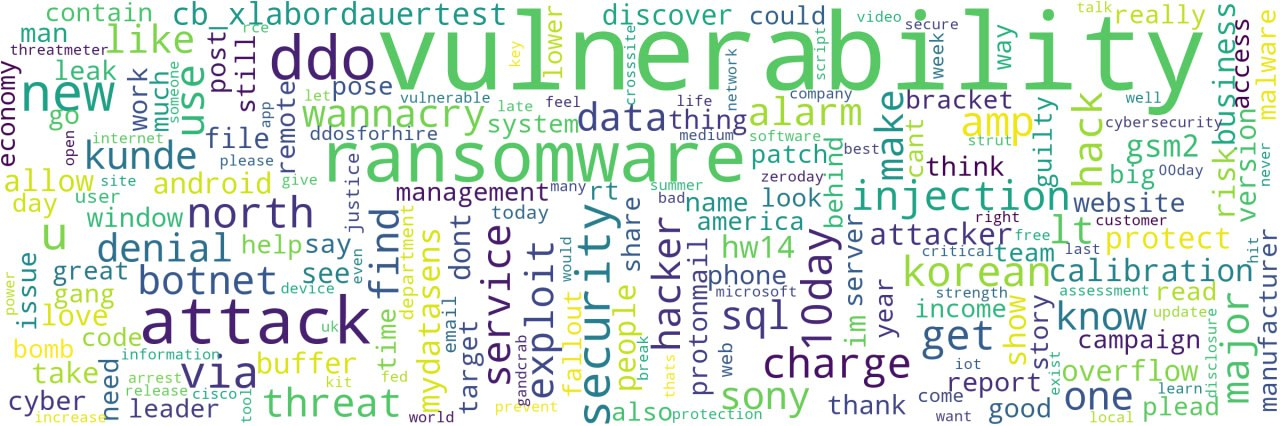
\includegraphics[width=1\linewidth]{Images/behzadan_wordcloud2}
    
\includegraphics[width=0.0625\linewidth]{Images/sep}
    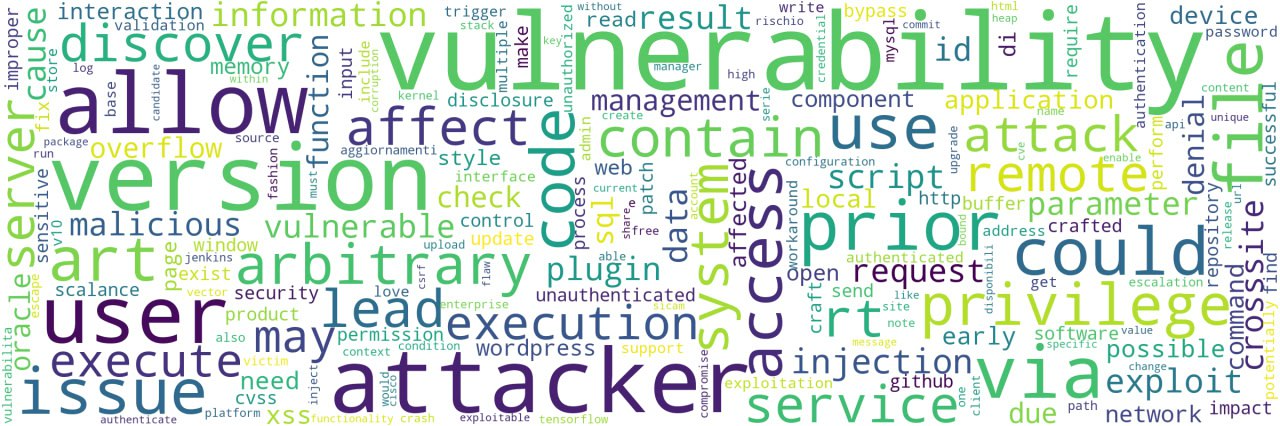
\includegraphics[width=1\linewidth]{Images/cotov_wordcloud}
    \caption{\textbf{Wordclouds} of the CyberPosts Dataset (top) and NistPosts Dataset (down).}
    \label{fig:wordclouds}
\end{figure}

By plotting the word clouds of the two datasets in Figure~\ref{fig:wordclouds}, the CyberPosts dataset shows more keywords related to cybersecurity topics than the NistPosts dataset. To quantify these differences, word distributions were plotted. The vocabulary overlap analysis showed that CyberPosts contained frequent words directly related to cybersecurity (e.g., \texttt{vulnerability}, \texttt{ransomware}, \texttt{attack}, \texttt{ddos}, \texttt{exploit}, \texttt{security}, \texttt{injection}, \texttt{sql}) for both the relevant and irrelevant posts. In contrast, NistPosts had way fewer cybersecurity-related words in the irrelevant posts, with the frequent words being more generic (e.g., \texttt{art}, \texttt{style}, \texttt{love}, \texttt{fashion}, \texttt{good}, \texttt{like}).

\begin{figure}
    \centering
    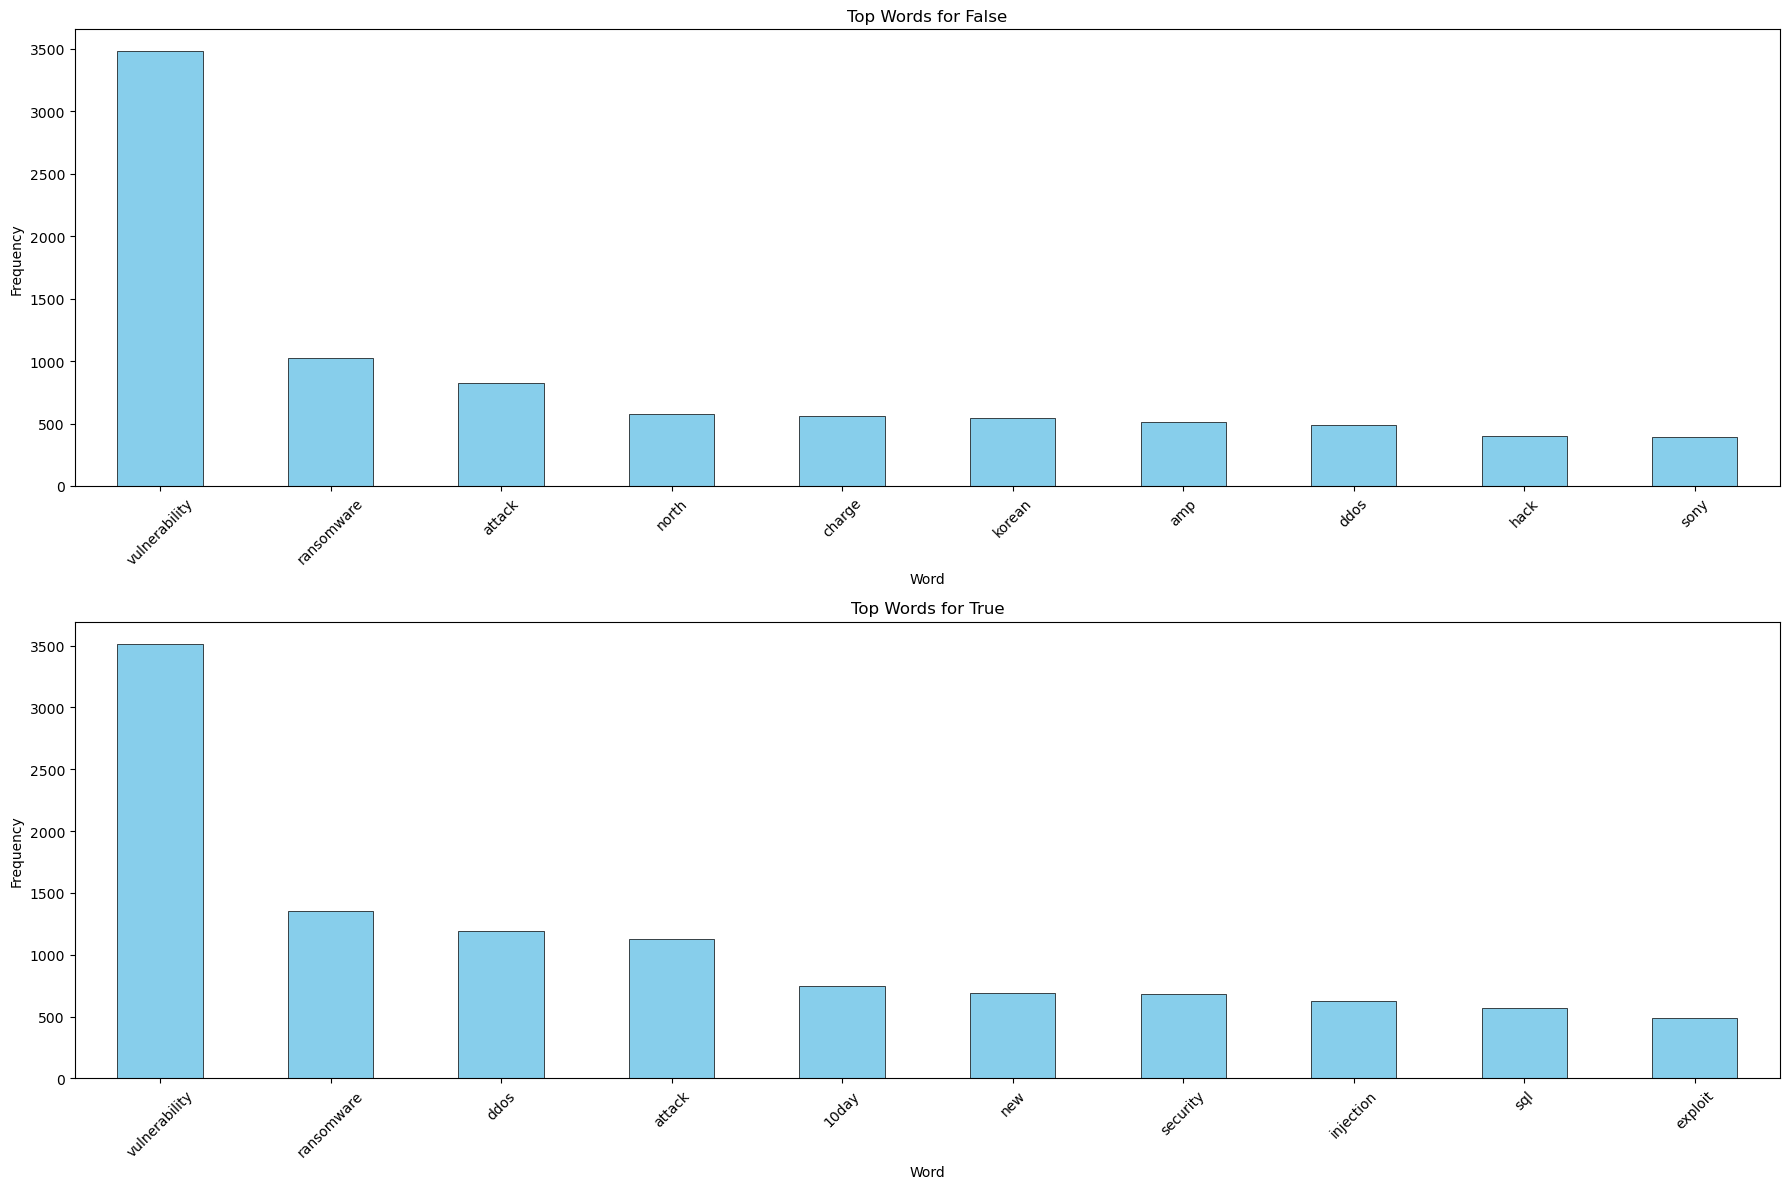
\includegraphics[width=1\textwidth]{Images/behzadan_words_distribution}
    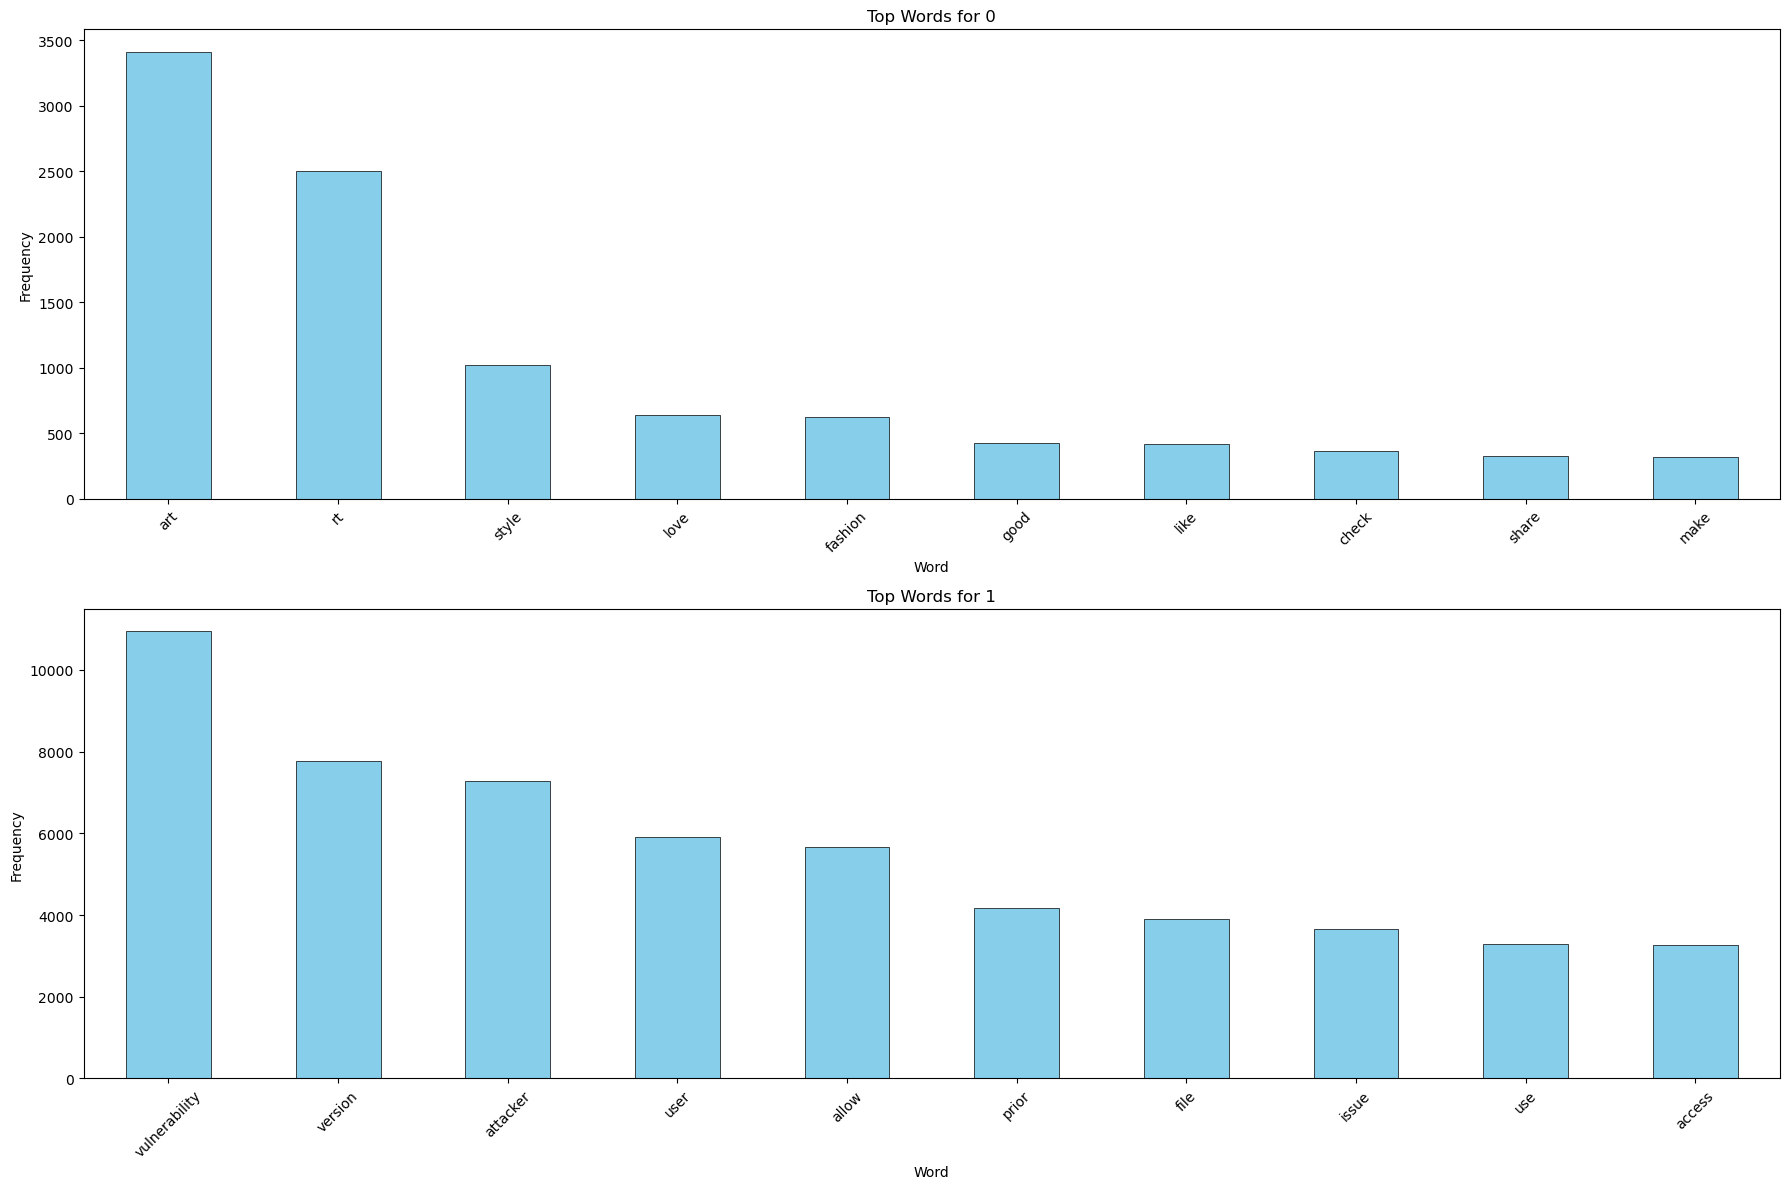
\includegraphics[width=1\textwidth]{Images/cotov_words_distribution}
    \caption{\textbf{Words Distribution} in CyberPosts Dataset (top) and NistPosts Dataset (down).}
    \label{fig:words-distribution}
\end{figure}

Figure~\ref{fig:words-distribution} shows that in CyberPosts, both relevance labels (0 and 1) contained a significant proportion of cybersecurity-related terms, making it a more suitable dataset for training a cybersecurity filter. In contrast, NistPosts showed a higher imbalance where label 0 (non-relevant) consisted of primarily non-cybersecurity terms, and label 1 (relevant) contained cybersecurity-related terms.

Even if the wordclouds (Figure~\ref{fig:wordclouds}) showed that some common keywords were evenly distributed, the word distribution analysis showed an imbalanced distribution across the two labels. For this reason, the classifiers were trained using the CyberPosts dataset to ensure they would be more robust in learning the post's underlying patterns. Ultimately, the NistPosts dataset was used as a second evaluation set to validate the models.

The CyberPosts dataset has different columns that can interest the implementation of a classifier; however, for obvious reasons, this study uses the ``\texttt{text}'' column, the ``\texttt{relevant}'' column for training and testing the binary classifier filter, and the ``\texttt{watson}'' column for training and testing the multi-label classifier model for assigning categories to posts. The ``\texttt{annotation}'' field is another interesting column since it contains the labeling of cybersecurity experts. Still, it was not used since its values were not considered essential for linking the posts to the nodes of companies' system graphs.

\begin{figure}
    \centering
    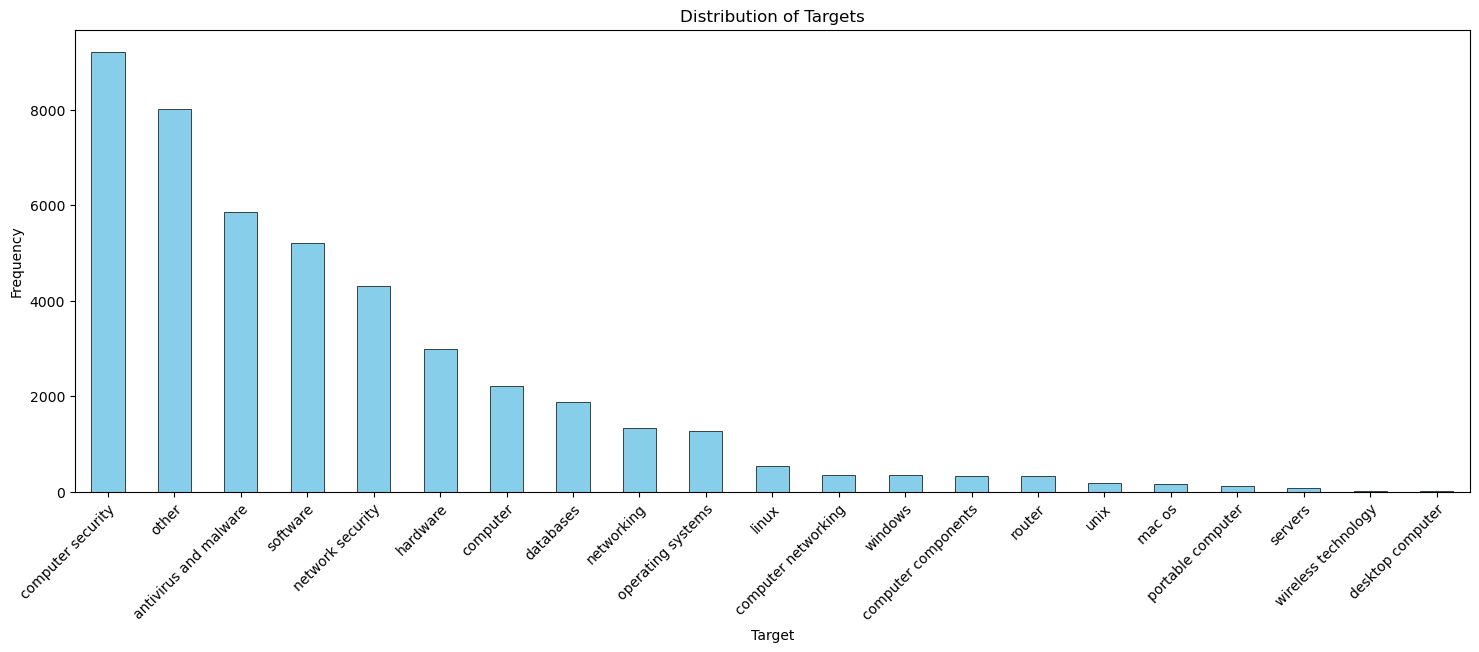
\includegraphics[width=1\linewidth]{Images/behzadan_target_distribution}
    \caption{\textbf{Distribution of Categories in CyberPosts Dataset}.}
    \label{fig:cyber-posts-target-distribution}
\end{figure}

A weak point of the CyberPosts dataset is its strongly imbalanced dataset for the MLC task (Figure~\ref{fig:cyber-posts-target-distribution}). The most common label among the posts is ``\texttt{Computer Security},'' with 9,216 samples associated. Then, at the second position, there is the ``\texttt{Other}'' label with 8,013 samples, which already highlights the imbalance. Still, in the third position, the label ``\texttt{Antivirus and Malware}'' with 5,854 samples, followed by the label ``\texttt{Software}'' with 5,214 samples, half of the most common label.


\section{Architecture}\label{sec:architecture}
\begin{figure}
    \centering
    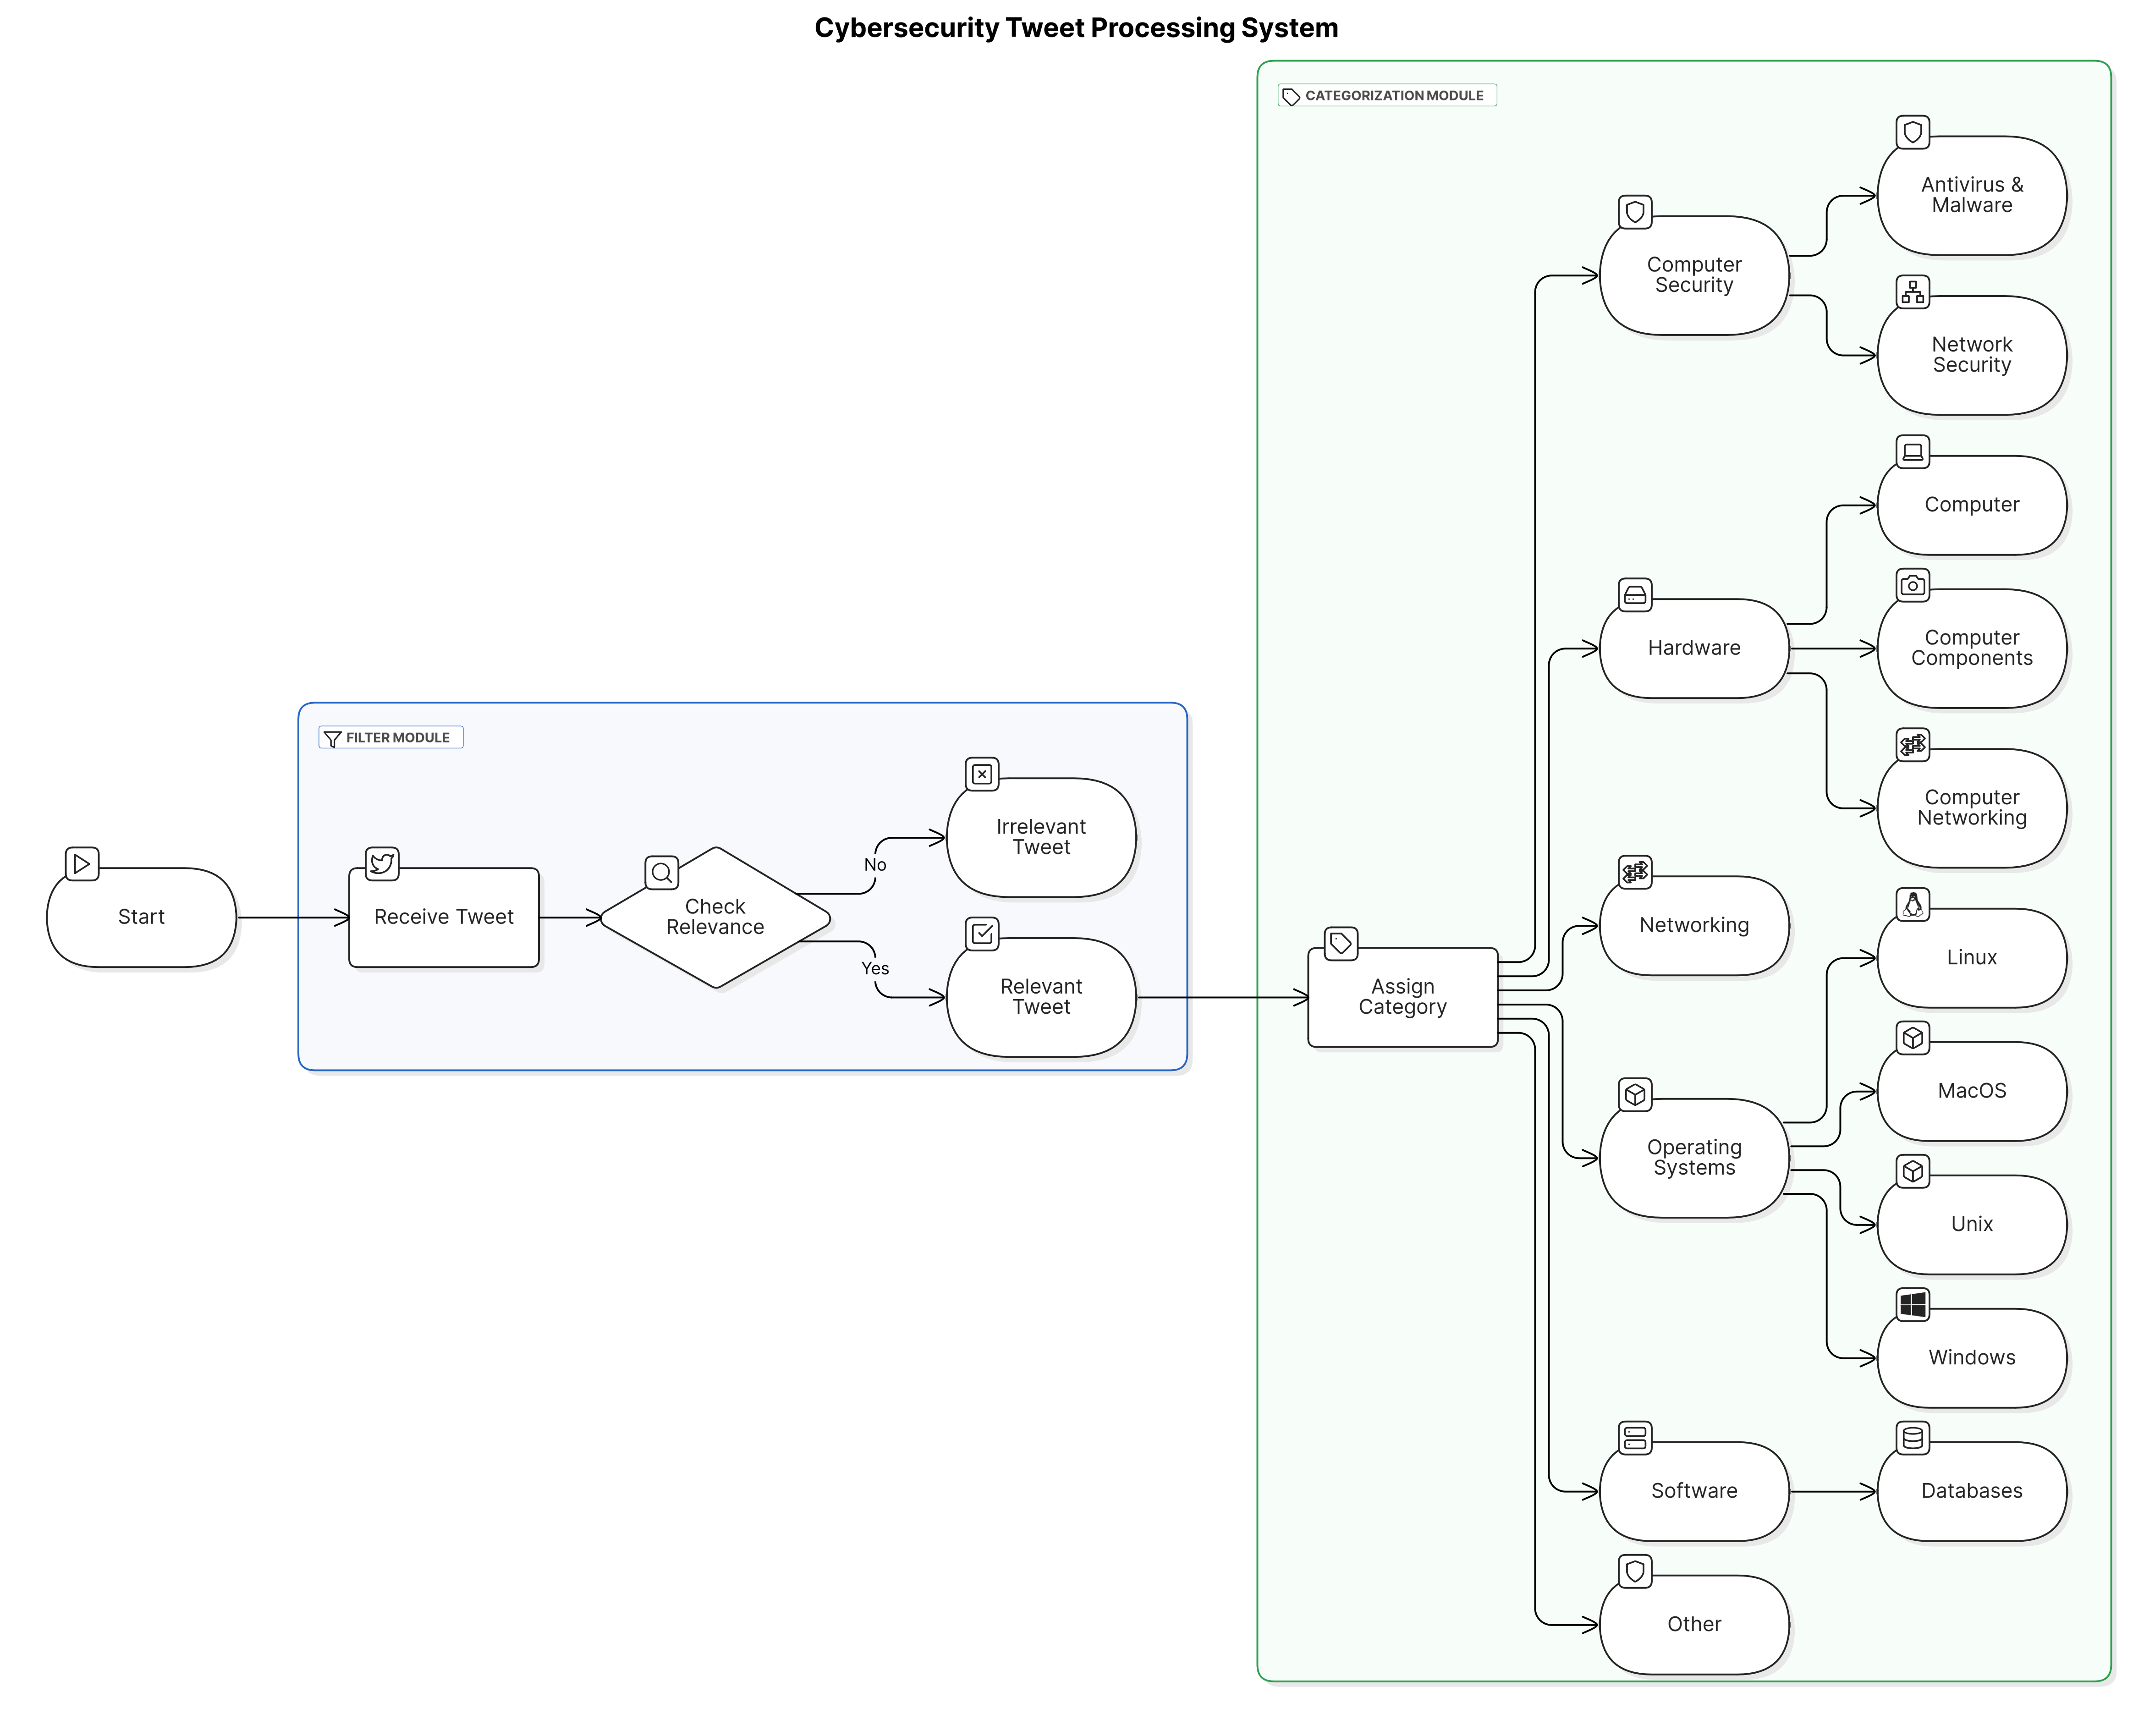
\includegraphics[width=\linewidth]{Images/system-schema-horizontal-new}
    \caption{\textbf{The Two-Step System's Architecture}.}
    \label{fig:two-step-system}
\end{figure}

The proposed system is a hierarchical multi-label classification approach. It operates in two structured levels: an initial classification into broad categories and a secondary classification into subcategories when applicable. This architecture ensures an interpretable classification process and enhances the precision of the multi-label classification predictions.

Once the categories are fixed, a deterministic mapping is applied to the list to map each category to a node type in system graphs.



\subsection{The Two-Step System}\label{subsec:two-step-system-mth}
In the Two-Step System, there are two modules: the \textit{Filter module} filters out all the posts irrelevant to cybersecurity topics, and the \textit{Categorization module} assigns hierarchical categories to each post considered relevant for end users.

Figure~\ref{fig:two-step-system} visually presents the system flow. Incoming posts are preprocessed by removing URLs, emails, mentions, and hashtags. Then, the embeddings are computed for each post, and the binary classification models predict its relevance. Then, the second module assigns categories to the posts predicted as relevant. The Categorization module is formed by two layers of models that classify posts into high-level categories (\texttt{Computer Security}, \texttt{Hardware}, \texttt{Networking}, \texttt{Operating Systems}, \texttt{Other}, and \texttt{Software}), and then classify posts into subcategories within the high-level categories, if applicable, as follows:

\begin{itemize}
    \item \texttt{Computer Security} $\rightarrow$ \texttt{Antivirus and Malware}, \texttt{Network Security}
    \item \texttt{Hardware} $\rightarrow$ \texttt{Computer}, \texttt{Computer Components}, \texttt{Computer Networking}
    \item \texttt{Operating Systems} $\rightarrow$ \texttt{Linux}, \texttt{MacOS}, \texttt{Unix}, \texttt{Windows}
    \item \texttt{Software} $\rightarrow$ \texttt{Databases}
\end{itemize}

For example, if a post is classified under \texttt{Hardware}, it is re-evaluated for the specific subcategories like \texttt{Computer Components}. If no subcategory is applicable, the classification remains in the high-level category.

\subsection{The One-Step System}\label{subsec:one-step-system}
The One-Step System integrates Filtering and Categorization modules to increase the filter's performance and avoid error propagation into the category classifier. In this case, the CyberPosts target for the MLC task was manipulated by forcing the irrelevant posts to have category ``\texttt{Other}'', so in the training phase, the models will learn to predict a category whenever the post is relevant, and ``\texttt{Other}'' otherwise. So, the system consists of five primary models trained to classify posts into high-level categories and subcategories, like the Two-Step System.

For example, given a list of posts, each post is processed by the embeddings and encoders. Then the models predict the categories among the high-level categories -- \texttt{Computer Security}, \texttt{Hardware}, \texttt{Networking}, \texttt{Operating Systems}, \texttt{Other}, and \texttt{Software}. As already said, the significant advantage of the One-Step System is that the filter and categorization modules are trained together because they are part of the same model. Consequently, when a post is recognized as irrelevant by the first layer category classifier, the model will assign only the category ``\texttt{Other}'' to the post, and the second layer category classifier will not be involved in the prediction. For all the relevant posts, the system will predict not only the high-level category but also the subcategories, and most importantly, it will not assign category ``\texttt{Other}'' to the relevant posts since it is forced to predict a category whenever the post is relevant.

\section{Implementation and Setup}\label{sec:implementation-and-setup}
In this section, the architecture implementation described in Section~\ref{sec:architecture} is presented, detailing the datasets used, the data preprocessing steps, the embedding models, the classification models, and the evaluation metrics employed to assess the models' performance.

\subsection{Datasets}\label{subsec:datasets-imp-stp}
\begin{figure}
    \centering
    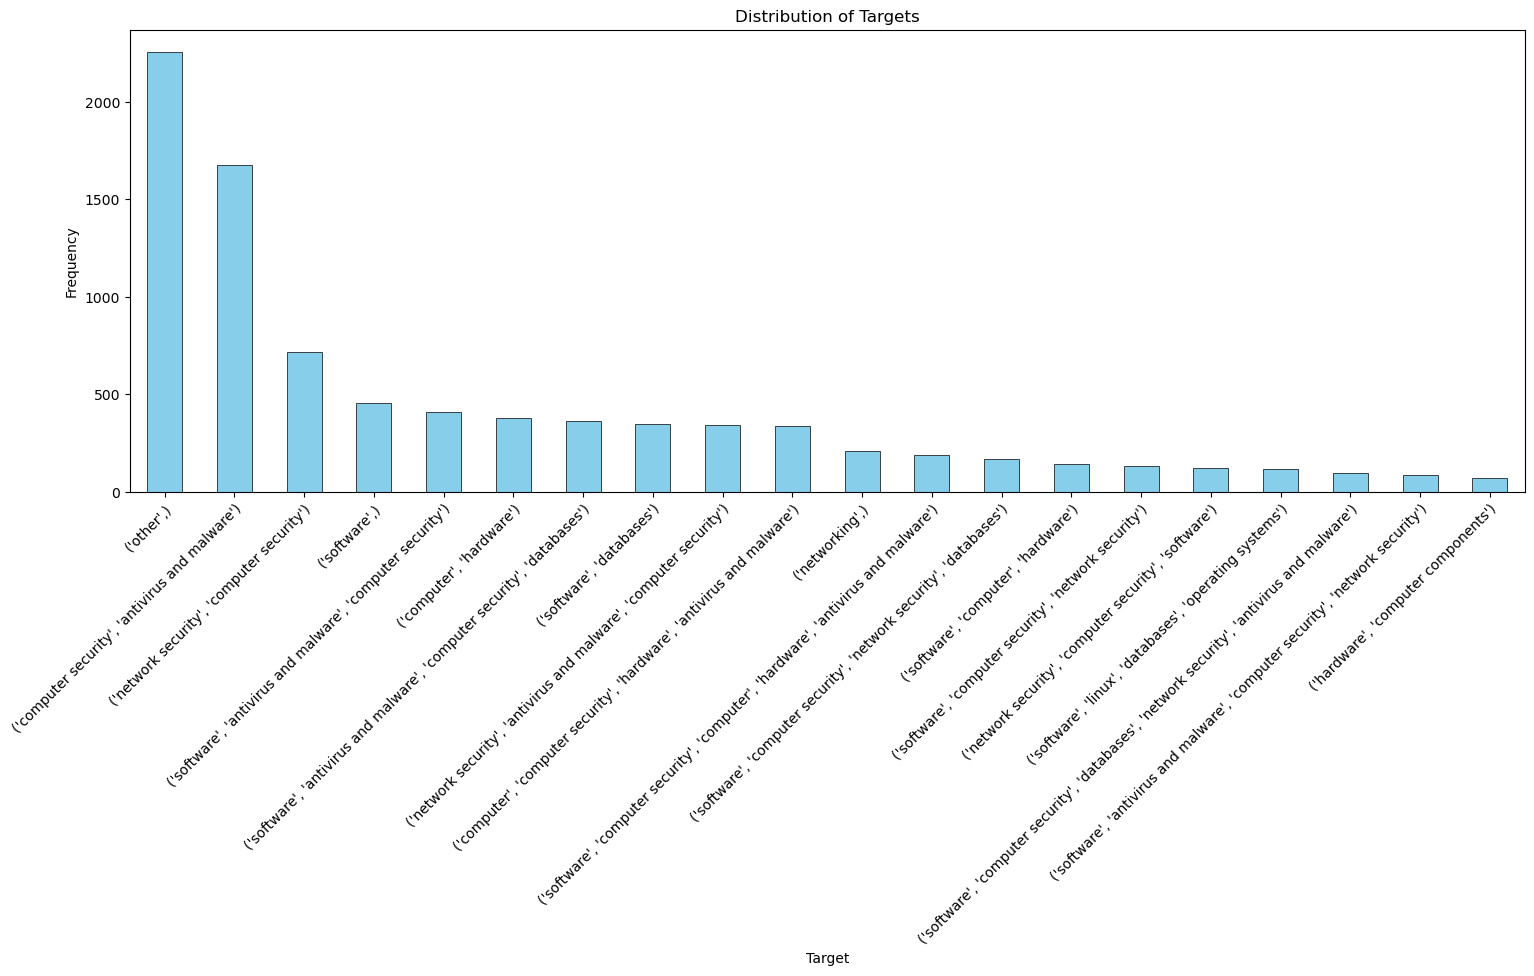
\includegraphics[width=1\linewidth]{Images/behzadan_target_set_distribution}
    \caption{\textbf{Distribution of Label-Sets in CyberPosts Dataset}.}
    \label{fig:cyber-posts-target-set-distribution}
\end{figure}

Since the CyberPosts dataset is strongly imbalanced, as highlighted in Figure~\ref{fig:cyber-posts-target-distribution}, the models have many difficulties generalizing the information to new unseen data. Another plot that helps understand the challenges in training for methods such as the Label Powerset algorithm is the Figure~\ref{fig:cyber-posts-target-set-distribution}, where the label-set ``\texttt{(Other)}'' is the most common with 2,255 samples, followed by ``\texttt{(Computer Security, Antivirus and Malware)}'' with 1,674 samples and ``\texttt{(Network Security, Computer Security)}'' with 719 samples.

Because of the distributions in Figure~\ref{fig:cyber-posts-target-distribution} and Figure~\ref{fig:cyber-posts-target-set-distribution}, it was expected to have higher performances with methods that did not consider the label dependencies, like the Binary Relevance algorithm, and lower performances with methods that considered the label dependencies, like the Label Powerset algorithm.

\subsection{Data Preprocessing}\label{subsec:data-preprocessing}
With the choice of not enhancing the posts with external information but the embeddings and encoders, there were defined models that only received text embeddings, so the embedding models had prior roles in the success of the training steps.

Before feeding the texts to the embeddings, a data cleaning process was performed to remove all the noises from the posts. In particular, the emails, URLs, mentions, and hashtags were removed since they were not considered informative for the posts.

For the training of the binary classification models, the posts were split into training and testing sets with an 80{\%} and 20{\%} ratio, respectively. The split was performed with the \texttt{train\_test\_split} function from the \texttt{scikit-learn} library by stratifying the data to ensure that the distribution of the classes was the same in both the training and testing sets.

The datasets for training and evaluating the multi-label classification models depended on the architecture used. For the Two-Step System, the data were filtered to retain only the posts relevant to cybersecurity topics, independently of the predictions of the filter modules. For the One-Step System, the data were manipulated to force the irrelevant posts to have the category ``\texttt{Other}'', so all the posts were used to train the models.

For the training of the two multi-label classification architectures, the posts were split into training and testing sets with an 80{\%} and 20{\%} ratio, respectively. In this case, the label sets were stratified to ensure that the distribution of the label sets was the same in both the training and testing sets. However, the label sets were poorly distributed in the dataset, so the split required discarding the samples associated with rare label sets. In particular, only the posts with label sets with at least 20 samples were considered for the training and testing split.


\subsection{Embeddings Models}\label{subsec:embeddings-models}
Across the experiments, the embeddings and encoders presented in Section~\ref{subsubsec:the-embeddings} were used: the embeddings to convert the posts into numerical vectors and the encoders to compute the post embeddings.

The chosen GloVe{\footnote{\href{https://nlp.stanford.edu/projects/glove/}{GloVe: Global Vectors for Word Representation}}} embeddings contained six billion tokens. Whenever words were not in GloVe's vocabulary, they were discarded as they were translated into zero vectors. It was the same for all the GloVe versions, namely the 50, 100, 200, and 300-dimensions. Ideally, the 50-dimension embeddings only captured the general text semantics. Still, they should not be informative enough for tasks such as assigning categories potentially correlated to each other in computer science. For this reason, it was expected to notice higher performances with the 300-dimensional embeddings among all the four static embeddings.

Since static embeddings are not generally used in state-of-the-art natural language processing applications, the encoders were applied to compute the post embeddings.

The SBERT{\footnote{\href{https://huggingface.co/sentence-transformers/all-mpnet-base-v2}{sentence-transformers/all-mpnet-base-v2}}} and DistilRoBERTa{\footnote{\href{https://huggingface.co/sentence-transformers/all-distilroberta-v1}{sentence-transformers/all-distilroberta-v1}}} were the first to be tested. Finally, the ATT{\&}CK-BERT{\footnote{\href{https://huggingface.co/basel/ATTACK-BERT}{basel/ATTACK-BERT}}} encoder was employed to increase accuracies and robustness. All of them were computed with the \texttt{sentence-transformers} library in Python.

\subsection{Classification Models}\label{subsec:classification-models}
For the training of the \textbf{Filter module} of the Two-Step System, the binary classification models were used to predict the relevance of the posts.

There were constructed 28 models by combining the four embeddings presented in Section~\ref{subsubsec:the-embeddings} (GloVe 6B 50D, GloVe 6B 100D, GloVe 6B 200D, and GloVe 6B 300D), and three encoders presented in Section~\ref{subsubsec:the-encoders} (DistilRoBERTa, SBERT, and ATT{\&}CK-BERT) with the four base classifiers presented in Section~\ref{subsec:binary-classification} (Logistic Regression, Naïve Bayes, Random Forest, and XGBoost).

Each model was implemented as a simple \texttt{scikit-learn} pipeline with a standard scaler as the first layer and the classifier as the second layer. The standard scaler only normalizes the data by centering the mean of the embeddings to 0 and their variance to a unit standard deviation. This normalization technique helps the algorithms in learning more efficiently without the need for scaling factors.

The best model for the Filter module was selected based on the highest mean cross-validation accuracy, with a cross-validation of 5 folds. Once the model was identified, it was hyperparameter-tuned with a Bayesian optimization technique using the \texttt{hyperopt} library in Python.

In the \textbf{Categorization module} and for both the architectures, the algorithms used for the binary classification task could not solve the problem, as for Logistic Regression, or were inefficient, as for Naïve Bayes, so state-of-the-art methods for solving multi-label classification tasks were used.

The multi-label classifiers for assigning categories to relevant posts are built manually by following the pseudocode presented in \cite{zhang2014}. In this case, the methods used for facing the problem were the same as explained in Section~\ref{subsec:multilabel-classification} (BR, CLR, CC, LP, PSt, MBR, RAkEL, and HOMER), combined with each base classifier presented in Section~\ref{subsec:binary-classification}, for all the embeddings and encoders: there were trained more than 200 models.

The best model for the Categorization module was selected based on the highest macro F1 score.

\subsection{Evaluation Metrics}\label{subsec:evaluation-metrics}
Different metrics were used to assess all the models and extract only those relevant to solving the two tasks (filter and categorization). The metrics include:
\begin{itemize}
    \item \textbf{Accuracy}. It is the number of correct classification predictions divided by the total number of predictions.
    \item \textbf{Precision}. It is the proportion of all the model's positive classifications that are actually positive.
    \item \textbf{Recall} (or True Positive Rate, TPR). It is the proportion of all actual positives classified correctly as positives.
    \item \textbf{F1 score}. It is the harmonic mean of precision and recall. This metric balances the importance of precision and recall and is preferable to accuracy for class-imbalanced datasets. More broadly, when precision and recall are close in value, F1 will be close to their value. When precision and recall are far apart, F1 will be similar to whichever metric is worse.
    \item \textbf{AUC} (Area Under the ROC Curve). It represents the probability that the model will rank the positive higher than the negative if given a randomly chosen positive and negative example.
    \item \textbf{Hamming loss}. It is a metric that computes the fraction of wrong labels to the total number of labels. It is used in multi-label classification and penalizes only the individual labels. A lower Hamming loss indicates better performance.
    \item \textbf{Macro Averaging}. This approach independently computes metrics like precision, recall, and F1-score for each label and then averages them. It treats all labels equally, making it suitable when they are equally important, but it may not accurately reflect performance if label frequencies vary significantly.
    \item \textbf{Micro Averaging}. This approach globally computes metrics by aggregating contributions from all labels. This method is more sensitive to labels with higher frequencies and is beneficial when labels have varying importance or imbalance. Notably, in multi-class evaluation, micro F1 is equivalent to accuracy. 
    \item \textbf{Sample-based Averaging}. This approach computes metrics for each instance individually and averages these scores across all instances. It provides a balanced view of precision and recall at the instance level, offering a nuanced assessment of model performance.
    \item \textbf{Weighted Averaging}. This approach computes metrics that account for the imbalance in class distribution by considering each class's support (i.e., the number of true instances). This approach ensures that the performance metrics -- such as precision, recall, and F1-score -- reflect the contribution of each class proportionally to its occurrence in the dataset.
\end{itemize}

For the Two-Step System, the metrics were computed for the filter and Categorization modules to evaluate the system's performance comprehensively. For the One-Step System, the metrics were calculated for the whole system, as the Filter and Categorization modules were integrated into a single model.

In particular, for the aggregated performances of the Two-Step System, the metrics of the Categorization module were evaluated only on the relevant posts, so the irrelevant posts were not considered in the evaluation.
\chapter{Experimental Results}\label{ch:experimental-results}
This project aimed to build a system that organizes and sorts posts about cybersecurity to raise awareness of critical security issues. The system's design is shown in Figure~\ref{fig:two-step-system}. It consists of two main parts: one part filters out unimportant posts, and another sorts the critical posts into different categories. By identifying and highlighting relevant security information, this system helps focus attention on useful content from the vast repository of social media posts. The system was tested using a collection of posts focused on cybersecurity topics. Each part was evaluated to evaluate how well it worked independently, looking specifically at the filtering and categorizing functions. This chapter presents the results of these tests, focusing on how well the systems that make binary decisions and the systems that handle multiple categories performed.

The chapter is divided into the following sections:
\begin{itemize}
    \item Section~\ref{sec:binary-classifiers-evaluation} explains the performance of the binary classifiers used in the filtering part.
    \item Section~\ref{sec:multi-label-classification-problem} examines the performance of the categorizing part, discussing both the Two-Step System and the One-Step System in Sections~\ref{subsec:two-step-system} and~\ref{subsec:one-step-system-imp-and-rsl}.
    \item Section~\ref{subsec:one-step-attack-bert-system} compares the One-Step System with the One-Step ATT{\&}CK-BERT System.
\end{itemize}


\section{Binary Classifiers Evaluation}\label{sec:binary-classifiers-evaluation}
The binary classifiers were trained to implement the Filter module. The experiments run in this phase showed that the embeddings impacted the model's training.

\begin{table}
    \centering
    \begin{tabular}{cc}
        \begin{tabular}{r}
            \\
            \\
            GloVe      \\
            6B 50D     \\
            \\
            \\
            GloVe      \\
            6B 100D    \\
            \\
            \\
            GloVe      \\
            6B 200D    \\
            \\
            \\
            GloVe      \\
            6B 300D    \\
            \\
            \\
            Distil-    \\
            RoBERTa    \\
            \\
            \\
            SBERT      \\
            \\
            \\
            \\
            ATT{\&}CK- \\
            BERT       \\
            \\
        \end{tabular} & \begin{tabular}{c|c|c|c|c|c|c||}
                            \hline
                                        & Accuracy       & Precision      & Recall         & F1             & AUC            & CV Acc         \\
                            \hline
                            LR          & 74.51          & 74.58          & 77.73          & 76.12          & 83.71          & 74.98          \\
                            GNB         & 67.88          & 70.87          & 64.45          & 67.51          & 75.62          & 69.17          \\
                            \textbf{RF} & \textbf{79.33} & \textbf{81.61} & 77.62          & 79.56          & 87.26          & \textbf{79.64} \\
                            XGB         & 79.22          & 80.71          & \textbf{78.85} & \textbf{79.77} & \textbf{87.29} & 79.36          \\
                            \hline
                            LR          & 75.29          & 75.80          & 77.33          & 76.56          & 84.33          & 75.51          \\
                            GNB         & 66.97          & 68.62          & 67.27          & 67.94          & 75.25          & 68.17          \\
                            \textbf{RF} & 78.68          & \textbf{81.65} & 75.82          & 78.62          & 86.81          & \textbf{79.08} \\
                            XGB         & \textbf{79.05} & 80.99          & \textbf{77.90} & \textbf{79.42} & \textbf{87.16} & 78.98          \\
                            \hline
                            LR          & 77.03          & 78.23          & 77.39          & 77.81          & 85.53          & 76.85          \\
                            GNB         & 68.57          & 72.79          & 62.43          & 67.21          & 76.03          & 69.15          \\
                            \textbf{RF} & 78.99          & \textbf{81.81} & 76.38          & 79.00          & 87.07          & \textbf{79.77} \\
                            XGB         & \textbf{79.53} & 81.25          & \textbf{78.74} & \textbf{79.98} & \textbf{87.48} & 79.62          \\
                            \hline
                            LR          & 76.90          & 78.33          & 76.83          & 77.57          & 85.84          & 77.59          \\
                            GNB         & 66.62          & 74.86          & 52.25          & 61.54          & 76.43          & 67.46          \\
                            \textbf{RF} & 79.20          & \textbf{82.19} & 76.32          & 79.15          & 86.99          & \textbf{79.77} \\
                            XGB         & \textbf{79.26} & 81.40          & \textbf{77.78} & \textbf{79.55} & \textbf{87.43} & 79.75          \\
                            \hline
                            LR          & 79.06          & 80.41          & 78.97          & 79.68          & 87.98          & 79.39          \\
                            GNB         & 76.78          & 75.79          & \textbf{81.89} & 78.72          & 84.48          & 76.85          \\
                            \textbf{RF} & \textbf{81.37} & \textbf{82.58} & 81.33          & \textbf{81.95} & 88.73          & \textbf{81.21} \\
                            XGB         & 80.44          & 81.29          & 81.10          & 81.19          & \textbf{88.79} & 80.62          \\
                            \hline
                            LR          & 79.83          & 80.81          & 80.31          & 80.56          & 88.10          & 79.01          \\
                            GNB         & 77.27          & 75.89          & \textbf{83.18} & 79.37          & 84.52          & 77.22          \\
                            \textbf{RF} & \textbf{81.16} & \textbf{82.76} & 80.48          & \textbf{81.61} & \textbf{88.94} & \textbf{81.34} \\
                            XGB         & 80.75          & 82.32          & 80.15          & 81.22          & 88.79          & 80.34          \\
                            \hline
                            LR          & 79.73          & 80.57          & 80.48          & 80.53          & 87.60          & 78.56          \\
                            GNB         & 77.06          & 77.20          & 79.58          & 78.37          & 84.08          & 76.20          \\
                            \textbf{RF} & \textbf{81.27} & \textbf{82.69} & 80.88          & 81.77          & 88.77          & \textbf{80.96} \\
                            XGB         & 81.19          & 82.26          & \textbf{81.38} & \textbf{81.82} & \textbf{89.08} & 80.45          \\
                            \hline
                            \hline
                        \end{tabular} \\
    \end{tabular}
    \caption{\textbf{Performances of Binary Classifiers} over test set of , with \texttt{CV = 5}.}
    \label{tab:filter-module}
\end{table}

The Table~\ref{tab:filter-module} shows that some classifiers, like Random Forest (RF) and XGBoost (XGB), work better than others, such as Logistic Regression (LR) and Gaussian Naïve Bayes (GNB). RF and XGB have higher accuracy, F1 scores, and AUC values with all text data types. This means these methods use advanced techniques that handle complex text relationships well.

The text representation, called embeddings, also influences model performance. For example, GloVe, a static embedding, slightly improves accuracy when the data representation size increases, raising accuracy from 74.51{\%} to 76.90{\%}. However, context-aware embeddings achieve the best results. They provide higher accuracy (around 81{\%}) and F1 scores (around 81{\%} and 82{\%}) for RF and XGB. Conversely, GNB struggles with complex data, showing lower recall and F1 scores, especially with more significant GloVe embeddings. GNB assumes all features are independent, which isn't always true in text data.

AUC values, indicating how well models differentiate between things, are high, between 83{\%} and 89{\%} for all models and embeddings. This means the models effectively distinguish different texts, even if their accuracy varies. In areas like cybersecurity, where understanding text nuances is essential, context-aware embeddings outperform static ones by more effectively capturing crucial details and security clues.

These results are particularly significant in the context of cybersecurity awareness. The high-performing models can effectively identify posts containing valuable security information, ensuring that critical advisories and updates reach those who need them while filtering out irrelevant content that might otherwise overwhelm security professionals and interested users.


\section{Multi-Label Classification Problem}\label{sec:multi-label-classification-problem}

\subsection{The Two-Step System}\label{subsec:two-step-system}
The \textbf{Two-Step System} architecture in Figure~\ref{fig:two-step-system} has a strong filtering module but struggles with multi-label classification for some specific categories. The filtering module uses a carefully tuned version of the Random Forest model, trained with SBERT embeddings. You can find details about the base classifier in Table~\ref{tab:filter-module}. This module is good at removing posts that are not relevant and showing high precision and recall. It achieves an F1-score of 82.3{\%}, an AUC of 81.8{\%}, and an accuracy of 81.8{\%}.

\begin{table}
    \centering
    \begin{tabular}{|r|rrrrr||}
        \hline
        \textbf{Category}     & \textbf{Precision} & \textbf{Recall} & \textbf{F1-Score} & \textbf{AUC} & \textbf{Support} \\
        \hline
        Antivirus And Malware & 0.65               & 0.79            & 0.71              & 0.76         & 857              \\
        Computer              & 0.61               & 0.38            & 0.47              & 0.67         & 318              \\
        Computer Components   & 0.00               & 0.00            & 0.00              & 0.50         & 35               \\
        Computer Networking   & 0.00               & 0.00            & 0.00              & 0.50         & 64               \\
        Computer Security     & 0.84               & 0.75            & 0.79              & 0.79         & 1164             \\
        Databases             & 0.00               & 0.00            & 0.00              & 0.50         & 314              \\
        Hardware              & 0.82               & 0.38            & 0.52              & 0.68         & 429              \\
        Linux                 & 0.00               & 0.00            & 0.00              & 0.50         & 94               \\
        Mac Os                & 0.00               & 0.00            & 0.00              & 0.50         & 30               \\
        Network Security      & 0.00               & 0.00            & 0.00              & 0.50         & 415              \\
        Networking            & 0.83               & 0.34            & 0.48              & 0.67         & 176              \\
        Operating Systems     & 0.94               & 0.58            & 0.71              & 0.79         & 227              \\
        Other                 & 0.51               & 0.84            & 0.63              & 0.81         & 472              \\
        Software              & 0.86               & 0.65            & 0.74              & 0.80         & 822              \\
        Unix                  & 0.11               & 0.73            & 0.20              & 0.84         & 22               \\
        Windows               & 0.00               & 0.00            & 0.00              & 0.50         & 72               \\
        \hline
        \hline
        Micro Avg             & 0.70               & 0.54            & 0.61              & 0.75         & 5511             \\
        Macro Avg             & 0.39               & 0.34            & 0.33              & 0.64         & 5511             \\
        Weighted Avg          & 0.61               & 0.54            & 0.56              & 0.72         & 5511             \\
        Samples Avg           & 0.67               & 0.59            & 0.61              & 0.77         & 5511             \\
        \hline
        \hline
    \end{tabular}
    \caption{\textbf{Performances of Two-Step System in Categorization Task}.}
    \label{tab:two-step-system}
\end{table}

The performance of the Two-Step System, shown in Table~\ref{tab:two-step-system}, highlights significant issues in multi-label classification, even with a strong filtering component. The filtering section performs well, achieving an F1-score of 82.3{\%}, AUC of 81.8{\%}, and accuracy of 81.8{\%}. However, the next step, which handles multi-label classification, shows inconsistent results across different categories.

A closer look at specific categories reveals a troubling pattern: six categories (``\texttt{Computer Components},'' ``\texttt{Computer Networking},'' ``\texttt{Databases},'' ``\texttt{Linux},'' ``\texttt{MacOS},'' ``\texttt{Windows},'' and ``\texttt{Network Security}'') have zero recall and F1-scores. This means the system fails to recognize these categories despite their presence in the test data. The system only does well in categories with a strong presence in the training data, such as ``\texttt{Computer Security}'' with an F1-score of 0.79 and ``\texttt{Antivirus and Malware}'' with an F1-score of 0.71.

The large gap between the micro-average F1 Score of 0.61 and the macro-average F1 Score of 0.33 shows that the system is biased towards majority classes and struggles with class imbalance. The weighted F1 Score of 0.56 also reflects this imbalance, leading to an overall accuracy of just 33.1{\%} for the whole classification task.

The main limitations of this system are the information loss during sequential processing, where errors in filtering affect the multi-label classification stage, and the inability to share learned information between the two tasks. The system also struggles with capturing relationships between labels, as seen in the stark performance differences between related categories. Finally, the system has difficulty handling class imbalance in the dataset, leading to poor recall for minority classes.

These limitations are significant in cybersecurity awareness contexts, where missing relevant security posts could result in overlooking critical vulnerabilities or threats. Ensuring comprehensive coverage across all security categories becomes essential when the goal is to raise awareness about cybersecurity issues. The One-Step System addresses these issues by integrating filtering and classification into a single framework. This approach removes the dependency on sequential steps and allows optimized model selection for each category. The One-Step System aims to overcome the information bottleneck in the Two-Step setup. Additionally, it handles class imbalance more effectively by using specialized models for minority classes, potentially improving recall for previously undetected categories.

\subsection{The One-Step System}\label{subsec:one-step-system-imp-and-rsl}
\begin{table}
    \centering
    \begin{tabular}{|r|rrrrr||}
        \hline
        \textbf{Category}     & \textbf{Precision} & \textbf{Recall} & \textbf{F1-score} & \textbf{AUC} & \textbf{Support} \\
        \hline
        Computer Security     & 0.94               & 0.43            & 0.59              & 0.70         & 1738             \\
        Antivirus and Malware & 0.92               & 0.52            & 0.66              & 0.75         & 1110             \\
        Network Security      & 0.91               & 0.26            & 0.40              & 0.63         & 817              \\
        Hardware              & 0.98               & 0.37            & 0.54              & 0.68         & 461              \\
        Computer              & 0.89               & 0.37            & 0.52              & 0.68         & 362              \\
        Computer Components   & 1.00               & 0.34            & 0.51              & 0.67         & 38               \\
        Computer Networking   & 1.00               & 0.37            & 0.54              & 0.68         & 38               \\
        Networking            & 0.79               & 0.33            & 0.46              & 0.66         & 240              \\
        Operating Systems     & 0.84               & 0.64            & 0.73              & 0.82         & 156              \\
        Linux                 & 0.88               & 0.73            & 0.79              & 0.86         & 77               \\
        Mac OS                & 1.00               & 0.54            & 0.70              & 0.77         & 13               \\
        Unix                  & 0.69               & 0.64            & 0.67              & 0.82         & 14               \\
        Windows               & 0.67               & 0.52            & 0.59              & 0.76         & 46               \\
        Other                 & 0.55               & 0.98            & 0.71              & 0.73         & 1603             \\
        Software              & 0.88               & 0.55            & 0.67              & 0.76         & 950              \\
        Databases             & 0.89               & 0.62            & 0.73              & 0.81         & 342              \\
        \hline
        \hline
        Micro Avg             & 0.74               & 0.55            & 0.63              & 0.76         & 8005             \\
        Macro Avg             & 0.86               & 0.51            & 0.61              & 0.74         & 8005             \\
        Weighted Avg          & 0.84               & 0.55            & 0.61              & 0.72         & 8005             \\
        Samples Avg           & 0.66               & 0.64            & 0.64              & 0.81         & 8005             \\
        \hline
        \hline
    \end{tabular}
    \caption{\textbf{Performances of One-Step System in Categorization Task}.}
    \label{tab:one-step-system}
\end{table}

Because the Two-Step System performed poorly, the One-Step System was developed to improve the classification of multiple labels.

The \textbf{One-Step System} results are shown in Table~\ref{tab:one-step-system}. It is designed to give the best performance for each label by using the model with the highest F1 score. This ensures that all labels are predicted accurately, enhancing the overall classification results.

The One-Step System achieves an overall accuracy of 58.91{\%} and a Hamming loss of 0.079. It shows strong performance in categories like ``\texttt{Linux}'' (F1-score: 0.79, AUC: 0.86) and ``\texttt{Operating Systems}'' (F1-score: 0.73, AUC: 0.82). However, it performs less well in categories such as ``\texttt{Network Security}'' (F1-score: 0.40, AUC: 0.63) and ``\texttt{Networking}'' (F1-score: 0.46, AUC: 0.66). The ``\texttt{Other}'' class has a high recall of 0.98, meaning it correctly identifies the most relevant instances, but its precision is lower at 0.55. Overall, the system achieves a weighted average F1-score of 0.61 and an AUC of 0.72, with a macro-averaged AUC of 0.74.

The system works by leveraging different models for labels, as each model might have unique strengths based on the label's characteristics. This approach spreads the prediction tasks across multiple models to reduce errors. Some models are better at handling security-related terms, while others excel at distinguishing between topics. Specific labels are more complex to predict because of imbalanced classes or similar meanings, like ``\texttt{Linux}'' and ``\texttt{Unix}.'' Using specialized models for particular labels helps the system adapt as needed. The system utilizes different models with various embeddings to effectively capture the most relevant information for predicting each category.

\begin{table}
    \centering
    \begin{tabular}{|r|rrrrr||}
        \hline
        \textbf{Label} & \textbf{Precision} & \textbf{Recall} & \textbf{F1-score} & \textbf{AUC} & \textbf{Support} \\
        \hline
        Not Relevant   & 0.81               & 0.93            & 0.87              & N/A          & 2444             \\
        Relevant       & 0.87               & 0.66            & 0.75              & N/A          & 1623             \\
        \hline
        \hline
        Accuracy       & -                  & -               & 0.83              & -            & 4067             \\
        Macro Avg      & 0.84               & 0.80            & 0.81              & 0.80         & 4067             \\
        Weighted Avg   & 0.83               & 0.83            & 0.82              & 0.80         & 4067             \\
        \hline
        \hline
    \end{tabular}
    \caption{\textbf{One-Step System's Performances in Filter Task}.}
    \label{tab:one-step-system-filter}
\end{table}

The system combines the Filter module with the Categorization module. So, it was checked how well the Filter submodule works by examining its predictions for the ``\texttt{Other}'' category.

Table~\ref{tab:one-step-system-filter} shows the system effectively distinguishes relevant from non-relevant posts. The Hamming Loss of 0.175 indicates the system makes few prediction errors. It has a high precision (0.87) for the ``\texttt{Relevant}'' class, which usually predicts correctly when identifying relevant posts. However, it has a recall of 0.66, meaning it sometimes misses relevant posts. For the ``\texttt{Not Relevant}'' class, the system has a strong F1-score of 0.87 due to its high recall (0.93), indicating it correctly identifies most non-relevant posts.

The balance between precision and recall shows the system focuses more on recall for the ``\texttt{Not Relevant}'' class. This means it tries hard to correctly identify non-relevant posts, reducing the chance of missing essential cybersecurity posts. The ``\texttt{Relevant}'' class has higher precision than recall, meaning it's usually right when it labels a post as relevant, even if it misses some relevant posts. This balance is essential in cybersecurity awareness, where including some non-important posts is preferable to missing crucial security advisories that could help users protect their systems and data. The macro-averaged F1-score of 0.81 and weighted F1-score of 0.82 show strong overall performance, confirmed by an 83{\%} accuracy rate.

\subsection{The One-Step ATT{\&}CK-BERT System}\label{subsec:one-step-attack-bert-system}
\begin{table}
    \centering
    \begin{tabular}{|r|rrrrr||}
        \hline
        \textbf{Category}     & \textbf{Precision} & \textbf{Recall} & \textbf{F1-score} & \textbf{AUC} & \textbf{Support} \\
        \hline
        Computer Security     & 0.94               & 0.43            & 0.59              & 0.70         & 1738             \\
        Antivirus and Malware & 0.92               & 0.52            & 0.67              & 0.75         & 1110             \\
        Network Security      & 0.91               & 0.26            & 0.41              & 0.63         & 817              \\
        Hardware              & 0.98               & 0.37            & 0.54              & 0.68         & 461              \\
        Computer              & 0.93               & 0.37            & 0.53              & 0.68         & 362              \\
        Computer Components   & 0.93               & 0.34            & 0.50              & 0.67         & 38               \\
        Computer Networking   & 1.00               & 0.47            & 0.64              & 0.74         & 38               \\
        Networking            & 0.79               & 0.33            & 0.46              & 0.66         & 240              \\
        Operating Systems     & 0.84               & 0.64            & 0.73              & 0.82         & 156              \\
        Linux                 & 0.88               & 0.73            & 0.79              & 0.86         & 77               \\
        Mac OS                & 1.00               & 0.54            & 0.70              & 0.77         & 13               \\
        Unix                  & 0.69               & 0.64            & 0.67              & 0.82         & 14               \\
        Windows               & 0.67               & 0.52            & 0.59              & 0.76         & 46               \\
        Other                 & 0.55               & 0.98            & 0.71              & 0.73         & 1603             \\
        Software              & 0.88               & 0.55            & 0.67              & 0.76         & 950              \\
        Databases             & 0.75               & 0.64            & 0.69              & 0.81         & 342              \\
        \hline
        \hline
        Micro Avg             & 0.73               & 0.56            & 0.63              & 0.76         & 8005             \\
        Macro Avg             & 0.85               & 0.52            & 0.62              & 0.74         & 8005             \\
        Weighted Avg          & 0.83               & 0.56            & 0.61              & 0.72         & 8005             \\
        Samples Avg           & 0.66               & 0.64            & 0.64              & 0.81         & 8005             \\
        \hline
        \hline
    \end{tabular}
    \caption{\textbf{Performances of ATT{\&}CK-BERT System in Categorization Task}.}
    \label{tab:attack-bert-system}
\end{table}

The \textbf{One-Step ATT{\&}CK-BERT System} is designed to sort posts into different categories using multiple models. These models are trained with ATT{\&}CK-BERT embeddings. Various methods are used to train each model to handle multiple categories simultaneously. The best-performing model for each category, based on a measure known as the macro F1 Score, is selected for the final system.

This system achieves a 58.77{\%} accuracy rate and a Hamming loss of 0.079. It performs exceptionally well in specific categories, with an F1 score of 0.79 for the ``\texttt{Linux}'' category. However, there are some trade-offs. In the ``\texttt{Other}'' category, it successfully identifies almost all relevant items (high recall of 0.98) but also includes many irrelevant ones (lower precision of 0.55). It does well in specific areas like ``\texttt{Operating Systems}'' (F1-score = 0.73) and ``\texttt{Databases}'' (F1-score = 0.69) but struggles with more ambiguous categories like ``\texttt{Network Security},'' which could be improved.

The ATT{\&}CK-BERT System shows the same overall accuracy and Hamming loss as the One-Step System, indicating similar errors in classifying each label. This suggests that using only ATT{\&}CK-BERT didn't significantly change the overall performance. The macro F1 Score is slightly better, meaning it performs better across all categories, especially those with fewer examples. However, the micro F1 Score, which focuses on individual cases, remains unchanged.

There's an improvement in recall in categories such as ``\texttt{Computer Networking}'' but a decrease in precision for ``\texttt{Databases},'' meaning more irrelevant items are included. Both systems perform similarly, though ATT{\&}CK-BERT does slightly better in the ``\texttt{Computer Security}'' subcategories. At the same time, precision drops for ``\texttt{Databases}'' and ``\texttt{Hardware}.'' Using only ATT{\&}CK-BERT embeddings doesn't significantly boost performance. A combination of ATT{\&}CK-BERT with other data representations provides a better balance between precision and recall, as seen in the One-Step System.

These findings have practical importance beyond just academic measurements. In real-world cybersecurity, accurately classifying technical information with high precision leads to better threat detection, improved information sorting, and less work for analysts. The results support the idea that a mix of embeddings is better than using a single type for handling the varied language in cybersecurity.

While specialized embeddings like ATT{\&}CK-BERT are useful, combining different embeddings provides a more effective solution for classifying cybersecurity text. This helps advance automated security information processing and can be applied to other specialized technical fields.

These findings have practical importance beyond just academic measurements. In raising cybersecurity awareness, accurately classifying technical information with high precision leads to better threat detection, improved information sorting, and less work for analysts trying to identify valuable security content from social media repositories. The results support the idea that a mix of embeddings is better than using a single type for handling the varied language in cybersecurity posts. This helps advance automated security information processing and can improve how we identify and highlight critical information for broader awareness.
\chapter{Conclusions}\label{ch:conclusions}
This thesis addressed the filtering and categorization of cybersecurity-related social media posts within the CS-Aware-Next project. Two architectures were built and compared on the same data: a Two-Step System that first filters the relevant posts and then categorizes them, and a One-Step System that categorizes all the posts with a single top-level model and implies relevance from the predicted categories. Both were developed on one grouped train-test split, with selection and tuning confined to the training partition, and evaluated once on the test partition with 95{\%} group-bootstrap confidence intervals.

The filter reaches a balanced accuracy of 0.787 (95{\%} interval from 0.769 to 0.808) and a ROC AUC of 0.876 (from 0.859 to 0.891) on the test set. The embedder of each component was selected by cross-validation, and the best one varies by component, with small differences among the candidates in the selection scores, so the choice should not be read as a ranking of the embedders. The categorization at the sub levels shows lower and wider-interval scores than the filter, and the labels there have a small support.

On the end-to-end comparison on the public labels, the micro F1 of the Two-Step System (0.651) and of the One-Step System (0.659) are not distinguishable: the paired difference is $-$0.007 with a 95{\%} interval from $-$0.030 to 0.011. The systems differ in the balance between precision and recall. The One-Step System has the higher micro precision (0.694 against 0.644), and the Two-Step System the higher micro recall (0.659 against 0.627). The recall of the Two-Step System is bounded by the recall of its filter, 0.798, since the relevant posts rejected by the filter lose their mapped labels. Which system is preferable therefore depends on the cost of a missed post relative to the cost of a false alert, and no claim of superiority is supported. The subset accuracy gives weak evidence in favour of the One-Step System ($-$0.020, interval from $-$0.042 to $-$0.001, without adjustment for multiple comparisons). Efficiency was not measured, and nothing is claimed about it. The evaluation on NistPosts, a dataset with a different annotation, is descriptive: both systems obtain high precision, and the One-Step System has the lower recall.

Several limitations qualify these findings. The results come from a single split, so they do not capture the variability due to the choice of the partition. The confidence intervals are conditional on the frozen trained systems and reflect only the resampling of the test posts. The category \texttt{Other} covers both the posts without a relevant category and the relevant posts without a mapped category, which affects the implicit relevance of the One-Step System and the interpretation of the public labels. The labels of the sub levels have a small support, so their estimates are wide. NistPosts follows a different annotation and cannot be used to compare the two systems on equal terms.

These limits suggest the directions for future work. Repeating the evaluation over several grouped splits, or nested resampling, would quantify the variability of the partition. A taxonomy that separates irrelevant posts from relevant posts without a mapped category would make the semantics of \texttt{Other} explicit. Additional annotated posts for the rare sub-level labels, or techniques designed for rare labels such as cost-sensitive learning, could improve their estimates. A decision threshold chosen for the desired balance of precision and recall would allow the operating point to be matched to an organization's needs, and a dedicated measurement of the computational cost would allow the two architectures to be compared on efficiency. Finally, annotating a second dataset with the same taxonomy would support a controlled evaluation of the generalization of both systems.


% --------------------------------------------------------------------------
% BIBLIOGRAPHY
% --------------------------------------------------------------------------

\addtocontents{toc}{\vspace{2em}} % Add a gap in the Contents, for aesthetics
\bibliography{Thesis_bibliography} % The references information is stored in the file named "Thesis_bibliography.bib."


% --------------------------------------------------------------------------
% APPENDICES
% --------------------------------------------------------------------------

\cleardoublepage
\addtocontents{toc}{\vspace{2em}} % Add a gap in the Contents, for aesthetics
\appendix


\chapter{Appendix A}\label{ch:appendix-a}
\section{Selection Diagnostics}\label{sec:selection-diagnostics}
This appendix reports the scores used to select the embedder and the per-label candidates of each categorization level (Section~\ref{subsec:classification-models}). They are computed out of fold on the training partition and are the maximum over many candidates: they are optimistic selection scores and must not be read as test results, which are reported in Chapter~\ref{ch:experimental-results}. The Filter selection diagnostics are in Table~\ref{tab:filter-module}.

\subsection{Embedder Selection}
Table~\ref{tab:oof-embedders} reports, for each level, the macro F1 of the composed out-of-fold predictions of each embedder; the selected embedder is the one with the highest value (in bold).

\begin{table}
    \centering
    \caption{\textbf{Composed out-of-fold macro F1 of each embedder} at each categorization level (selection scores on the training partition).}
    \label{tab:oof-embedders}
    \footnotesize
    \resizebox{\textwidth}{!}{\begin{tabular}{lccccccc}
        \hline
        \textbf{Level} & \textbf{GloVe 50D} & \textbf{GloVe 100D} & \textbf{GloVe 200D} & \textbf{GloVe 300D} & \textbf{DistilRoBERTa} & \textbf{SBERT} & \textbf{ATT{\&}CK-BERT} \\
        \hline
        Two-Step general & 0.549 & 0.534 & 0.568 & 0.582 & 0.596 & 0.598 & \textbf{0.607} \\
        Computer Security & 0.594 & 0.610 & \textbf{0.696} & 0.669 & 0.619 & 0.630 & 0.647 \\
        Hardware & 0.589 & 0.611 & 0.619 & 0.646 & 0.666 & \textbf{0.695} & 0.681 \\
        Operating Systems & 0.695 & 0.731 & 0.736 & 0.743 & \textbf{0.827} & 0.784 & 0.777 \\
        Software & 0.745 & 0.772 & 0.796 & 0.791 & \textbf{0.802} & 0.794 & 0.796 \\
        One-Step top level & 0.523 & 0.517 & 0.541 & 0.554 & 0.580 & \textbf{0.597} & 0.584 \\
        \hline
    \end{tabular}}
\end{table}

\subsection{Per-Label Candidates}
Table~\ref{tab:selected-candidates} lists, for each level, the candidate selected for each label with the selected embedder, written as method[base classifier] (BR, CLR, CC, LP, PSt, MBR, RAkEL, HOMER with the base classifiers LR, DT, and RF). The candidate of each label is the one with the highest pooled out-of-fold F1 on that label.

\begin{table}
    \centering
    \caption{\textbf{Selected candidate for each label} of each level.}
    \label{tab:selected-candidates}
    \footnotesize
    \begin{tabular}{lll}
        \hline
        \textbf{Level (embedder)} & \textbf{Label} & \textbf{Candidate} \\
        \hline
        Two-Step general (ATT{\&}CK-BERT) & Computer Security & RAkEL[RF] \\
         & Hardware & MBR[RF] \\
         & Networking & LP[LR] \\
         & Operating Systems & RAkEL[LR] \\
         & Other & HOMER[RF] \\
         & Software & HOMER[RF] \\
        \hline
        Computer Security (GloVe.6B.200D) & Antivirus and Malware & MBR[RF] \\
         & Network Security & MBR[RF] \\
         & Other & MBR[DT] \\
        \hline
        Hardware (SBERT) & Computer & CLR[RF] \\
         & Computer Components & MBR[LR] \\
         & Computer Networking & CC[LR] \\
         & Other & CLR[LR] \\
        \hline
        Operating Systems (DistilRoBERTa) & Linux & MBR[DT] \\
         & MacOS & LP[LR] \\
         & Other & RAkEL[LR] \\
         & Unix & HOMER[LR] \\
         & Windows & CLR[LR] \\
        \hline
        Software (DistilRoBERTa) & Databases & BR[LR] \\
         & Other & BR[RF] \\
        \hline
        One-Step top level (SBERT) & Computer Security & MBR[RF] \\
         & Hardware & MBR[RF] \\
         & Networking & PSt(pruning 25, 2 reintroduced)[LR] \\
         & Operating Systems & RAkEL[LR] \\
         & Other & CLR[RF] \\
         & Software & HOMER[RF] \\
        \hline
    \end{tabular}
\end{table}


%\chapter{Appendix B}\label{ch:mlcclasses}


% LIST OF FIGURES
\listoffigures

% LIST OF TABLES
\listoftables

% LIST OF SYMBOLS
% Write out the List of Symbols on this page
%    \chapter*{List of Symbols} % You have to include a chapter for your list of symbols (
%    \begin{table}[H]
%        \centering
%        \begin{tabular}{lll}
%            \textbf{Variable} & \textbf{Description} & \textbf{SI unit} \\\hline\\[-9px]
%            $\bm{u}$        & solid displacement   & m \\[2px]
%            $\bm{u}_f$        & fluid displacement   & m \\[2px]
%        \end{tabular}
%    \end{table}

% ACKNOWLEDGEMENTS

\cleardoublepage

\end{document}
